\documentclass[12pt,pdflatex]{article}
\usepackage{color}
\usepackage[usenames,dvipsnames]{xcolor}
\usepackage{colortbl} 
\usepackage{graphicx}
\usepackage{colordvi}
\usepackage{amssymb}
\usepackage{ulem}
\usepackage{graphicx}
\usepackage{caption}
\usepackage{subcaption}
\pagestyle{empty}
%\textheight 510pt
%\textwidth 683.4pt
%\oddsidemargin 0pt
%\evensidemargin 0pt
%\topmargin -82pt
%\fboxrule0.05in
%\fboxsep0.1in
\usepackage{fancyhdr}
\pagestyle{fancy}
\addtolength{\headheight}{2.5pt}
\lfoot{\thepage\ of \pageref{lastpage}}
%\cfoot{Rolf Andreassen}
\rfoot{University of Cincinnati} 

\newcommand{\mb}{\mathbf}
\boldmath 

\begin{document}
\begin{center}
{\LARGE Combining mixing results}
\end{center}

\section{Introduction}

The new $D^0\to K\pi$ result from LHCb provides a credibly powerful constraint
on mixing parameters. This note describes a fit in the style of HFAG to combine 
our result with previous measurements. 

\section{Chi-square calculation}

The purpose of our fit is to combine the errors on several different
measurements of the same parameters, where each measurement may have a
different relation to the underlying true mixing parameters (eg measuring
$(x'^2, y')$ in place of $(x, y)$), and where the numbers in each measurement
may be strongly correlated. To do so we construct an overall $\chi^2$ for
all the results:
\begin{eqnarray}
\chi^2 &=& \vec\epsilon^T \sigma^-1 \vec\epsilon
\end{eqnarray}
where the elements of $\vec\epsilon$ are given by
$\epsilon_i = m_i - p_i$. Here $\vec m$ is the list of measured
values from experiments, and $\vec p$ is a set of ``proposed'' values
for the mixing parameters; we use MINUIT to vary $\vec p$ so as
to minimise $\chi^2$. Finally, $\sigma$ is an $N\times N$ matrix where
$N$ is the number of measurements, with $\sigma_{ij} = e_i c_{ij} e_j$.
Here $e_i$ is the reported error on measurement $i$, and $c_{ij}$ is the
correlation coefficient between measurements $i$ and $j$. 

Notice that, if
the measurements are uncorrelated, then $\sigma$ reduces to
a diagonal matrix where the elements are the squares of the measurement
errors. In this case $\chi^2$ is simply the sum $\sum\limits_{i}\epsilon_i^2/e_i^2$,
that is, each element is the difference between a measurement
and the corresponding prediction, divided by the error on the measurement,
squared. In other words, if there are no correlations we recover
the usual chi-square goodness-of-fit metric. 

\section{Fit variants}

In full generality, we wish to fit for no less than seven underlying
related mixing parameters:
\begin{itemize}
\item $x$ and $y$, the normalised mass and width differences
\item $R_D^+$ and $R_D^-$, the ratios of rates
\item $\delta$, the strong phase difference
\item $|q/p$ and $\phi$, the magnitude and phase of the indirect CP violation. 
\end{itemize}
The observed inputs, however, are not all direct measurements of these
quantities. From $D^0\to K_S\pi\pi$ we get direct measurements of $x$, $y$, $|q/p|$ and $\phi$;
$D^0\to K\pi$ results also yield $R_D^\pm$ directly, although sometimes quoted
as $R_D = \frac{1}{2}(R_D^+ + R_D^-)$ and $A_D = \frac{R_D^+ - R_D^-}{R_D^+ + R_D^-}$.
However, we also measure the derived parameters $x'^{2(\pm)}$, $y'^{(\pm)}$, $y_{CP}$, and $A_\Gamma$,
defined as:
\begin{eqnarray}
x' &=& x\cos\delta + y\sin\delta \\
y' &=& y\cos\delta - x\sin\delta \\
x'^{\pm} &=& \left(\frac{1\pm A_M}{1\mp A_M}\right)^{1/4}\left(x'\cos\phi \pm y'\sin\phi\right) \\
y'^{\pm} &=& \left(\frac{1\pm A_M}{1\mp A_M}\right)^{1/4}\left(y'\cos\phi \mp x'\sin\phi\right) \\
2y_{CP}  &=& \left(|q/p|+|p/q|\right)y\cos\phi - \left(|q/p|-|p/q|\right)x\sin\phi\\
2A_\Gamma  &=& \left(|q/p|-|p/q|\right)y\cos\phi - \left(|q/p|+|p/q|\right)x\sin\phi\\
\end{eqnarray}
where the helper quantity $A_M$ is given by
\begin{eqnarray}
A_M &=& \frac{|q/p|^2 - |p/q|^2}{|q/p|^2 + |p/q|^2}. 
\end{eqnarray}

To calculate $\vec\epsilon$, then, we take in a vector of proposed mixing parameters
from MINUIT, calculate the resulting observable parameters from the equations above, 
and subtract the actually observed numbers.

In addition to the fully-general fit allowing all these variables to float, 
there are some variants imposing different no-CPV constraints:
\begin{itemize}
\item No CP violation. In this fit we set $|q/p|=1$, $\phi=0$, and $R_D^+=R_D^-$, 
and fit only for $x$, $y$, $\delta$, and $R_D$. 
\item No direct CP violation. With no direct CP violation, $R_D^+=R_D^-$;
in addition, the four parameters $x$, $y$, $\phi$ and $|q/p|$ are related 
(in the limit that CPV is small) by the constraint
%\begin{eqnarray}
%%|q/p| &=& 1 - \frac{y}{x}\tan\phi \\
%%\phi &=& \frac{x}{y}\atan\left(\frac{1-|q/p|^2}{1+|q/p|^2}\right)
%\end{eqnarray}
Thus we have two variants on this fit:
\begin{description}
\item[2a] Here we allow $|q/p|$ to float and calculate $\phi$
from the constraint. 
\item[2b] We allow $\phi$ to float and calculate $|q/p|$ from the constraint. 
\end{description}
\item All CPV allowed. As $A_D$ is quite
small, the contribution of a new physics phase to $\phi$ is far below
our current sensitivity; consequently the constraint above is a reasonable
approximation. We therefore run three variants of the all-CPV-allowed 
scenario:
\begin{description}
\item[3a] All parameters float, no constraint.
\item[3b] $\phi$ is calculated from $|q/p|$ as above, rather than allowed to float.
$R_D^+$ and $R_D^-$ are both free, as before.
\item[3c] As in 3b, but with $|q/p|$ calculated from the constraint and $\phi$ allowed
to float.
\end{description}
\end{itemize}

In addition, we do a fit not allowing direct CP violation, in which the
free parameters are $x_{12}$, $y_{12}$, and $\phi$

\section{Measurements used}



%\section{Results}
% Insert result section here. 
\section{Results}
\label{sec:Results}
The results are split into subsections depending on the type of CP Violation allowed.
Additonally, results are presented using a variety of different combinations of the
available data. Figure~\ref{fig:xy_nocpv_variations} shows all variations for the 
no CPV allowed fits. Figure~\ref{fig:xy_all_variations} shows the results for a 
subset of variations on All CPV allowed fits. 
\subsection{No CP Violation Allowed}
Table~\ref{table:nocpv_output_table} lists the results from the No CP Violation allowed
global fit. As $A_\Gamma =0$ in the the case of No CPV, the data is not included in 
this fit. Additionally, we take subsets of the data which do not include results from
Belle, BaBar and CDF in order to explore the change in $\chi^2/$ndf of the global fit.
\begin{table}[htdp]
%	\begin{scriptsize}

\begin{center}
\resizebox{16cm}{!}{
\begin{tabular}{|c||c||c||c||c|}
\hline
 & All Results & No BaBar $K\pi$& No Belle, BaBar $K\pi$ & No Belle, BaBar, CDF $K\pi$ \\ \hline
$x[\%]                    $ & $0.378\pm 0.180 $& $0.467\pm 0.183  $& $0.473\pm 0.186  $& $0.474\pm 0.187$ \\ \hline
$y[\%]                    $ & $0.629\pm 0.080 $& $0.649\pm 0.089  $& $0.651\pm 0.090  $& $0.655\pm 0.090$ \\ \hline
$\delta_{K\pi}[\text{deg}]$ & $9.334\pm 12.487$& $14.601\pm 10.694$& $14.902\pm 10.689$& $14.550\pm 10.730$ \\ \hline
$R_D[10^{-3}]             $ & $3.493\pm 0.039 $& $3.542\pm 0.044  $& $ 3.547\pm 0.047 $& $3.547 \pm 0.047$ \\ \hline
$\chi^2/ndf               $ & $43.8487/16     $& $27.8873/13      $& $24.343/10       $& $13.5119/7$ \\ \hline
\end{tabular}
}
\end{center}
\caption{Output values of No CPV allowed global fit. Different columns list subsets of
allowed data.}
\label{table:nocpv_output_table}
%\end{scriptsize}
\end{table}%

\begin{figure}[htb]
  \begin{center}
    \begin{subfigure}[b]{0.4\textwidth}
      \centering
      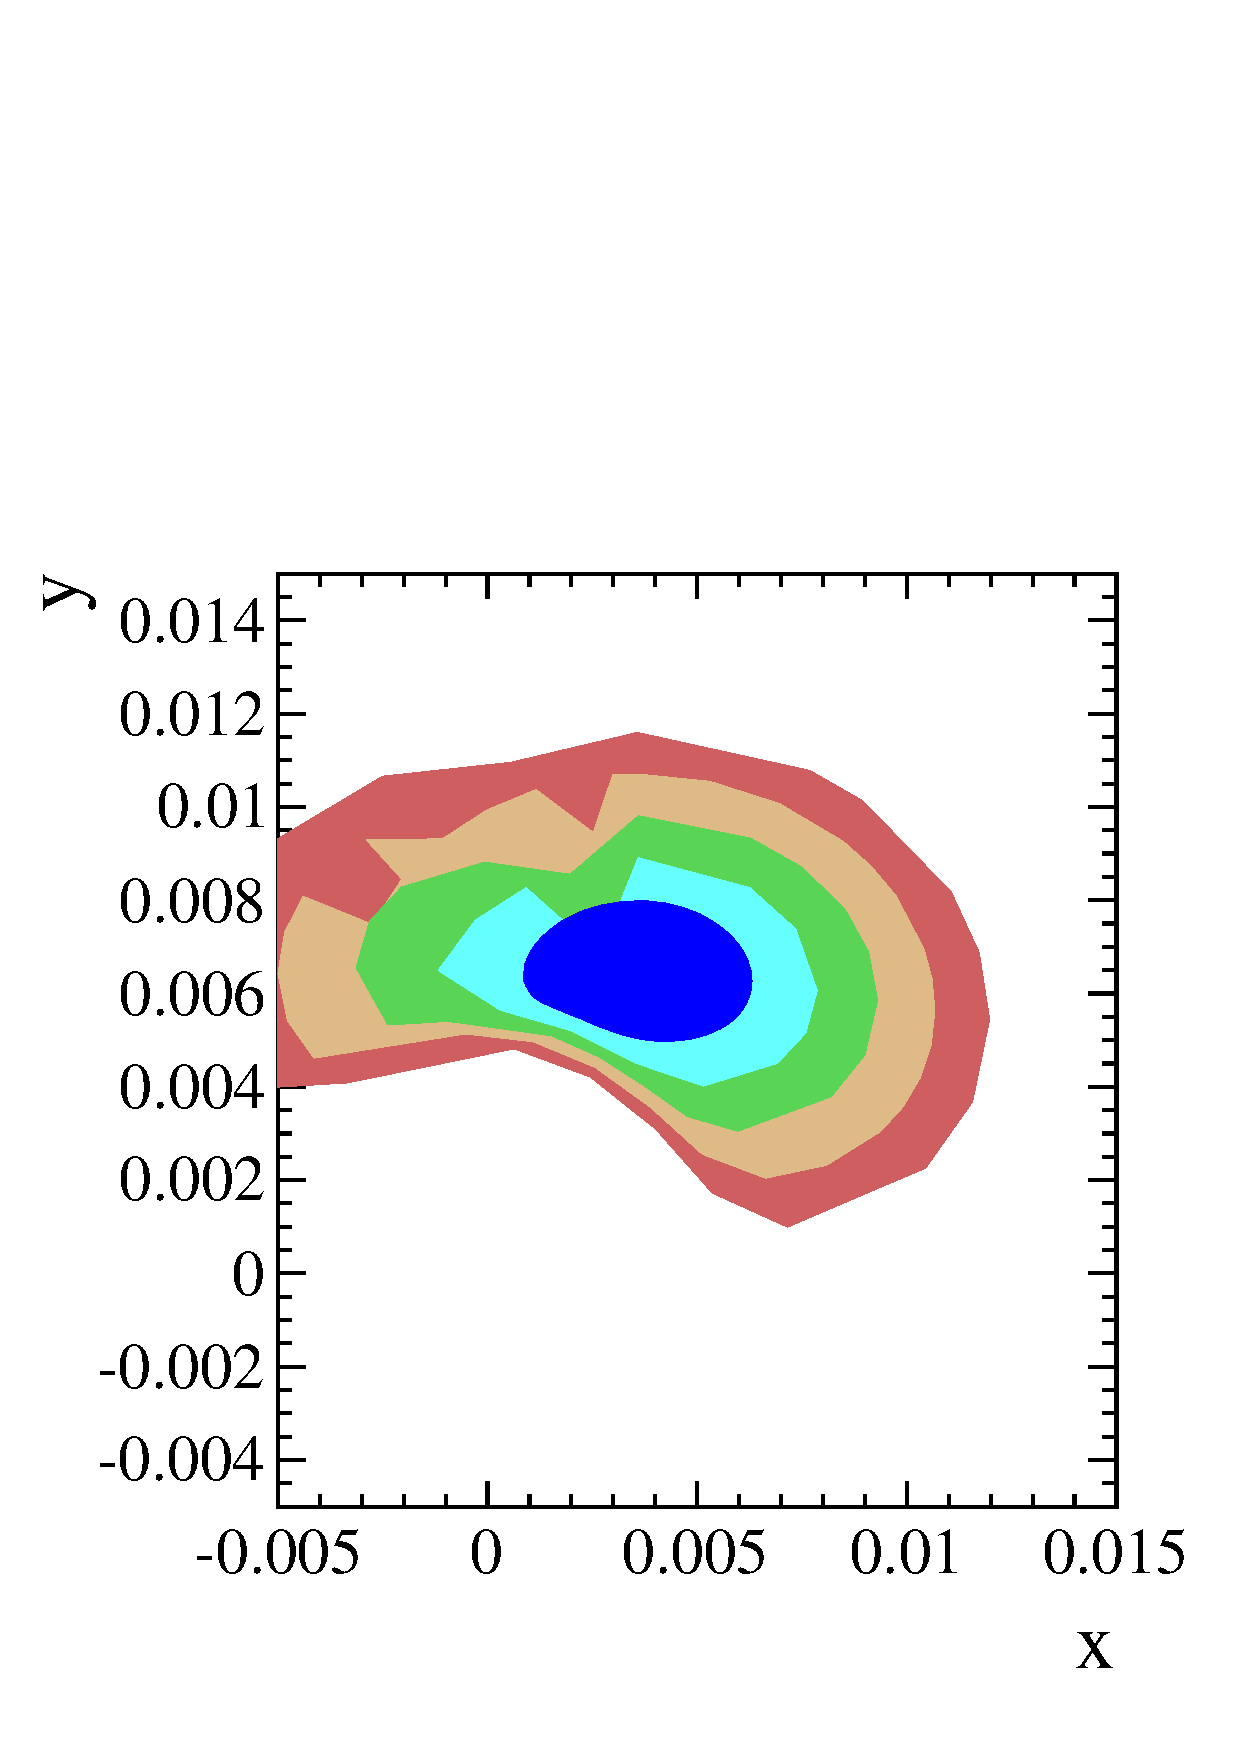
\includegraphics[width=\textwidth]{finalplot_nocpv__graph.pdf}
      \caption{Two dimensional error ellipses for x and y using all measurements listed in Table~\ref{table:nocpv_output_table}.}
      \label{fig:xy_no_cpv_}
    \end{subfigure}%
    \begin{subfigure}[b]{0.4\textwidth}
      \centering
      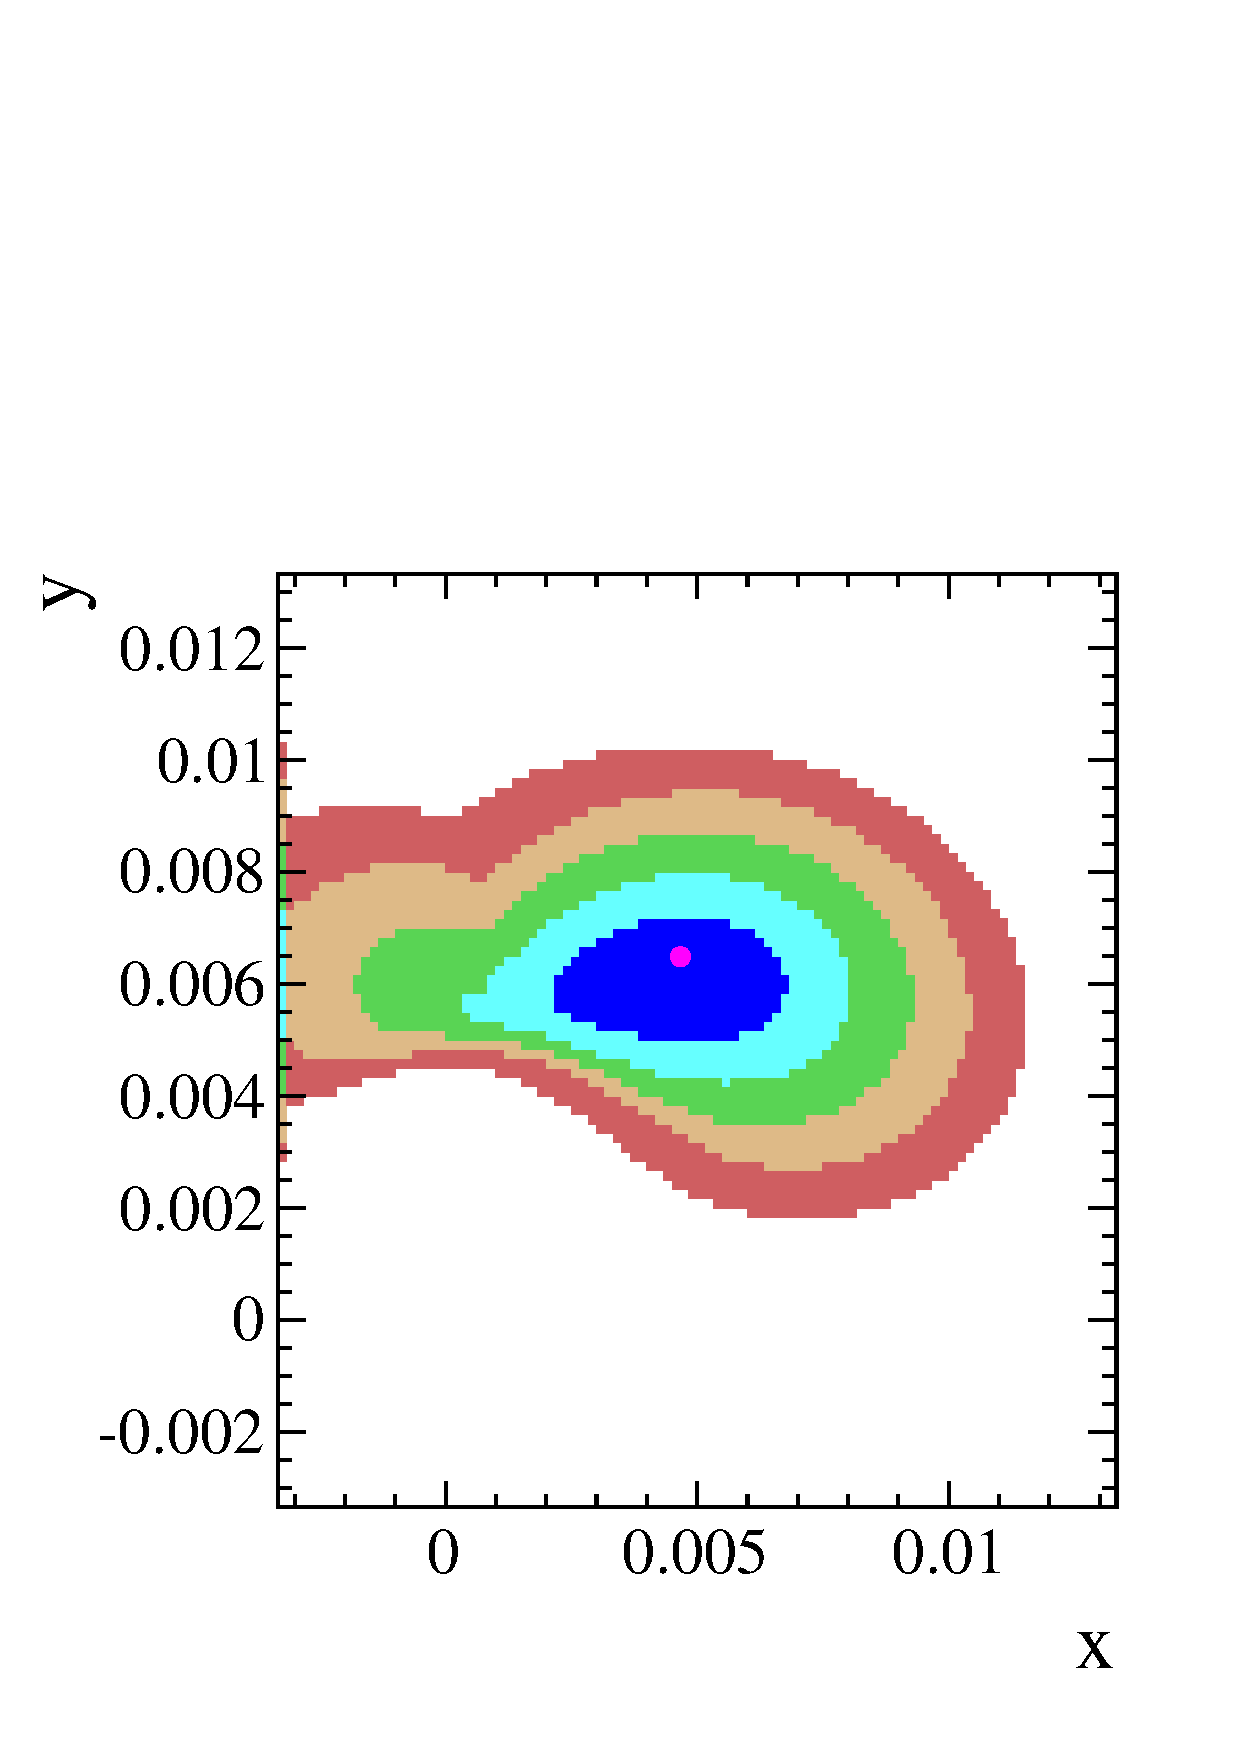
\includegraphics[width=\textwidth]{finalplot_nocpv__babar_graph.pdf}
      \caption{Two dimensional error ellipses for x and y using all available measurements except the .}
      \label{fig:xy_no_cpv_}
    \end{subfigure}%
    %\hspace{2mm}
    
    \begin{subfigure}[b]{0.4\textwidth}
      \centering
      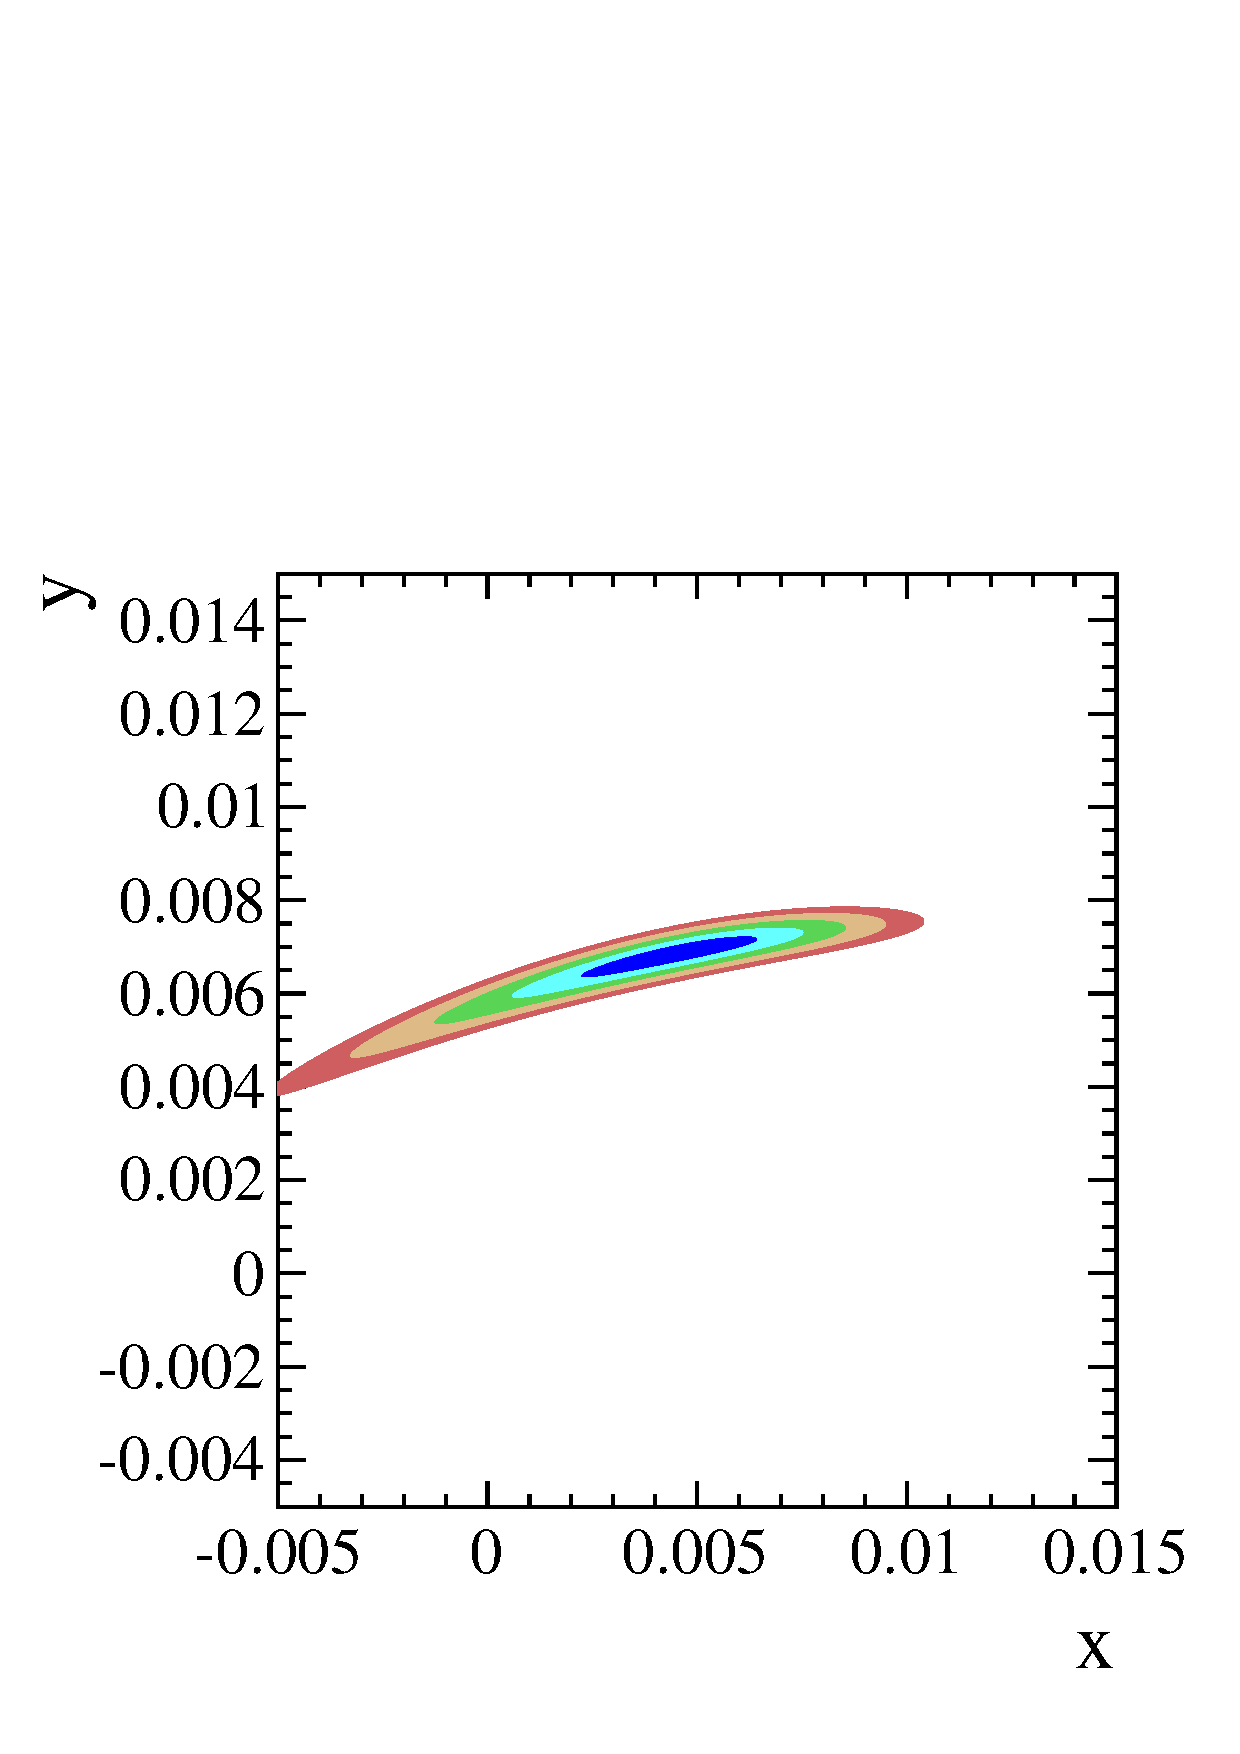
\includegraphics[width=\textwidth]{finalplot_nocpv__belle_babar_graph.pdf}
      \caption{Two dimensional error ellipses for x and y from fit excluding Belle and BaBar $K\pi$ results.}
      \label{fig:xy_no_cpv_nobelle_babar}
    \end{subfigure}%
    \hspace{2mm}
    \begin{subfigure}[b]{0.4\textwidth}
      \centering
      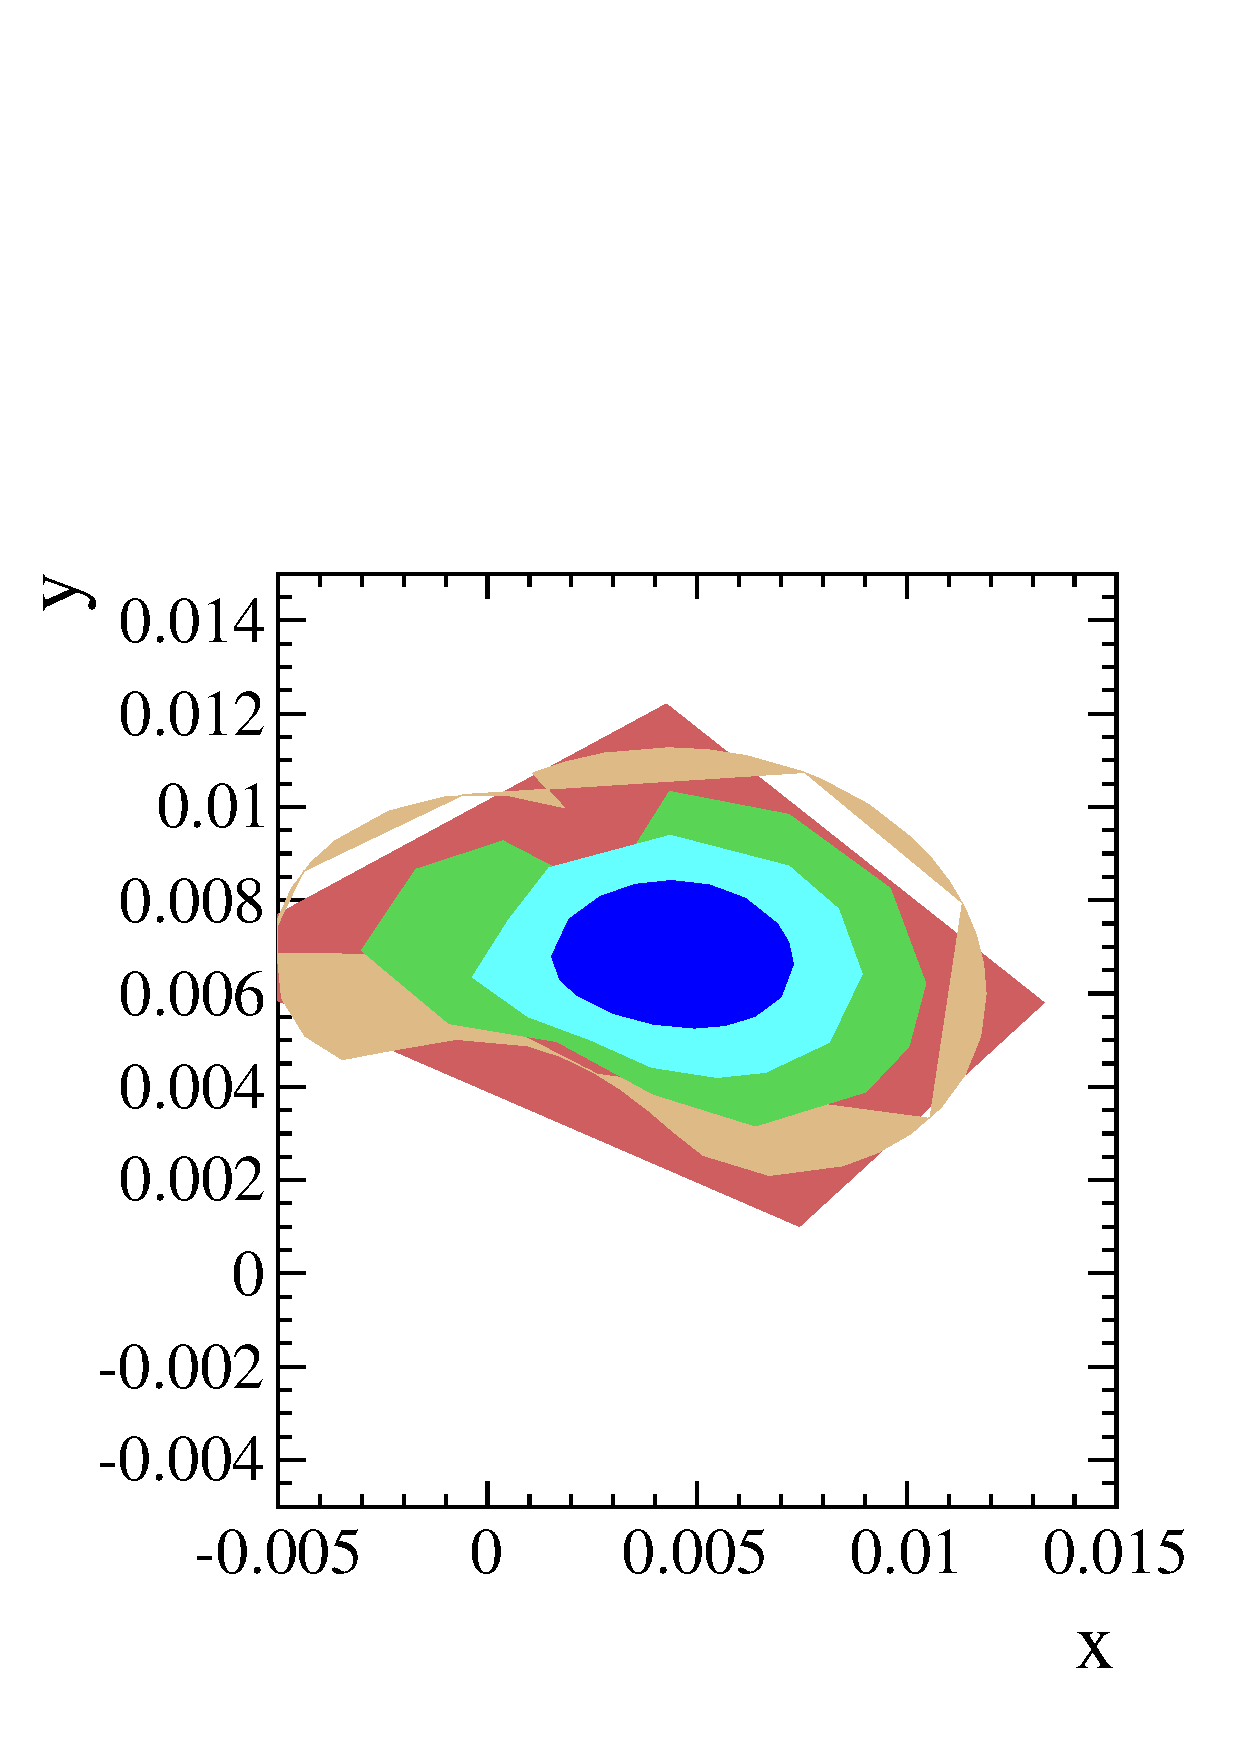
\includegraphics[width=\textwidth]{finalplot_nocpv__belle_babar_cdf_graph.pdf}
      \caption{Two dimensional error ellipses for x and y from fit excluding Belle, BaBar and CDF measurements.}
      \label{fig:xy_no_cpv_nocdf}
    \end{subfigure}%
    %\vspace*{-1.0cm}
  \end{center}
  \caption{Two dimensional error ellipses of $x$ and $y$ from fit for No CPV. Exclusion of the Belle and BaBar results drastically change the slope of the error ellipses. The differing colors represent the 1-5$\sigma$ contours.}
  \label{fig:xy_nocpv_variations}
\end{figure}
\subsection{No Direct CP Violation Allowed}
Table~\ref{table:nodcpv_output_table} lists the results of the global fit of no direct
CP violation. The final three columns of the table represent the effect of the 
inclusion of the preliminary LHCb $A_\Gamma$ result in the global fit.
The inlcusion of this result does not change the central values or errors substantially.


\begin{table}[htdp]
%\begin{tiny}

\begin{center}
\resizebox{16cm}{!} {
\begin{tabular}{|c||c||c||c||c|}
\hline
& All Measurements & No Belle, BaBar$K\pi$& No Belle, BaBar$K\pi$, add $A_{\Gamma\text{ LHCb}}$ & No Belle, BaBar, CDF $K\pi$, add $A_{\Gamma\text{ LHCb}}$ \\ \hline

$x(\times10^{-3})$ & $ 5.191\pm 1.746 $& $4.843\pm 1.782$& $4.845\pm1.782$& $4.844\pm1.787$ \\ \hline

$y(\times10^{-3})$ &$ 6.343\pm 0.905$ & $6.797\pm 1.029$& $6.797\pm 1.030$& $6.809\pm 1.031$ \\ \hline

$\delta_{K\pi}(\times10^{-1})[\text{rad}]$ &$2.468\pm 1.763$ & $3.187\pm 2.021$&$3.188\pm 2.021$ & $3.084\pm 2.040$ \\ \hline

$R_D(\times10^{-3})$ & $ 3.571\pm 0.046 $&$3.555\pm0.046$ & $3.556\pm 0.046$& $3.556\pm 0.047$ \\ \hline

$|q/p|(\times10^{-1})$ & $9.931 \pm 0.125$& $9.935\pm0.135$& $9.929\pm 0.131$ & $9.930\pm0.130 $\\ \hline

$\chi^2/ndf$ & 24.8569/28 & 19.0559/13& 19.3925/15& 8.61793/12\\ \hline

\end{tabular}
}
\end{center}
\caption{Output values of No Direct CPV allowed global fit. Different columns list 
subsets of allowed data.}
\label{table:nodcpv_output_table}
%\end{tiny}
\end{table}%



\begin{figure}[htb]
  \begin{center}
    \begin{subfigure}[b]{0.4\textwidth}
      \centering
      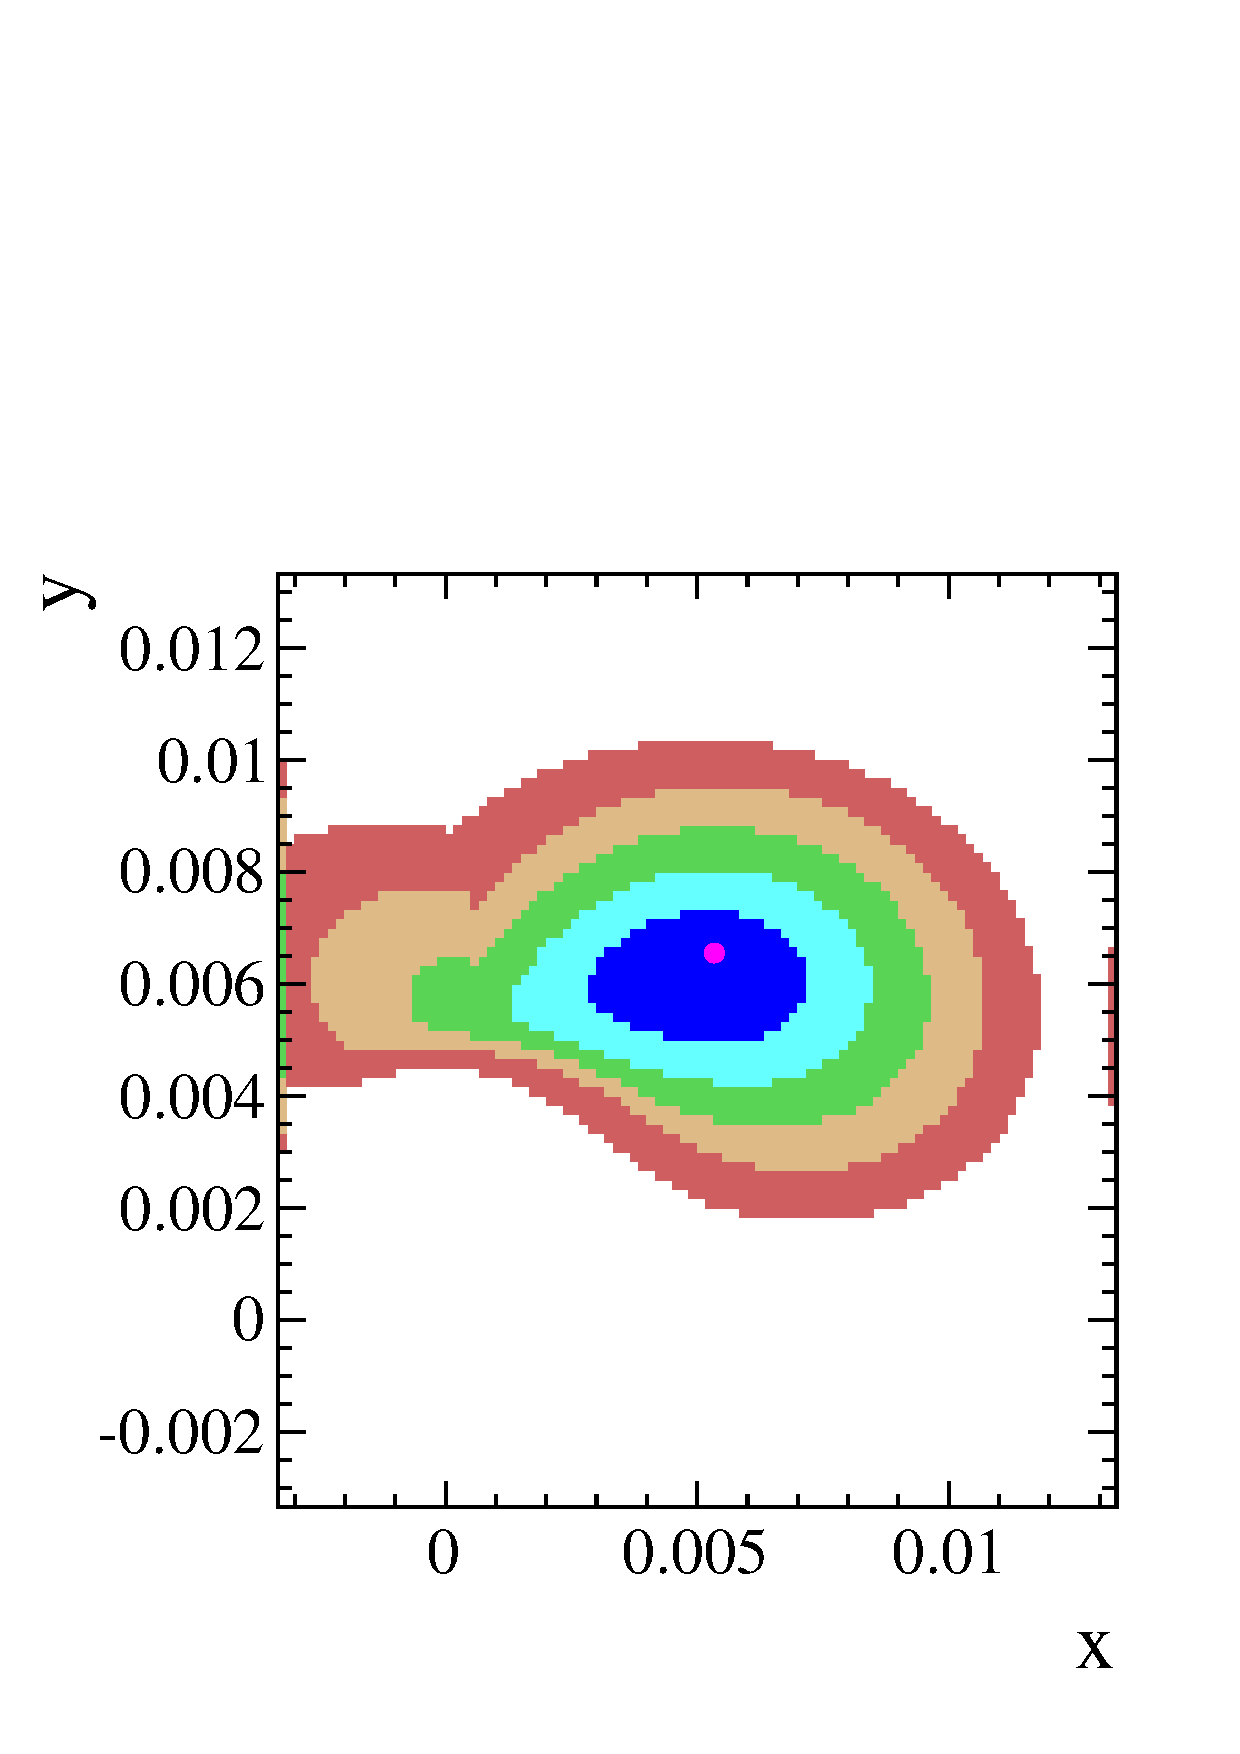
\includegraphics[width=\textwidth]{finalplot_nodcpv__.pdf}
      \caption{Two dimensional error ellipses for x and y from fit to all listed data.}
      \label{fig:all_nodcpv}
    \end{subfigure}%
    \hspace{2mm}
    \begin{subfigure}[b]{0.4\textwidth}
      \centering
      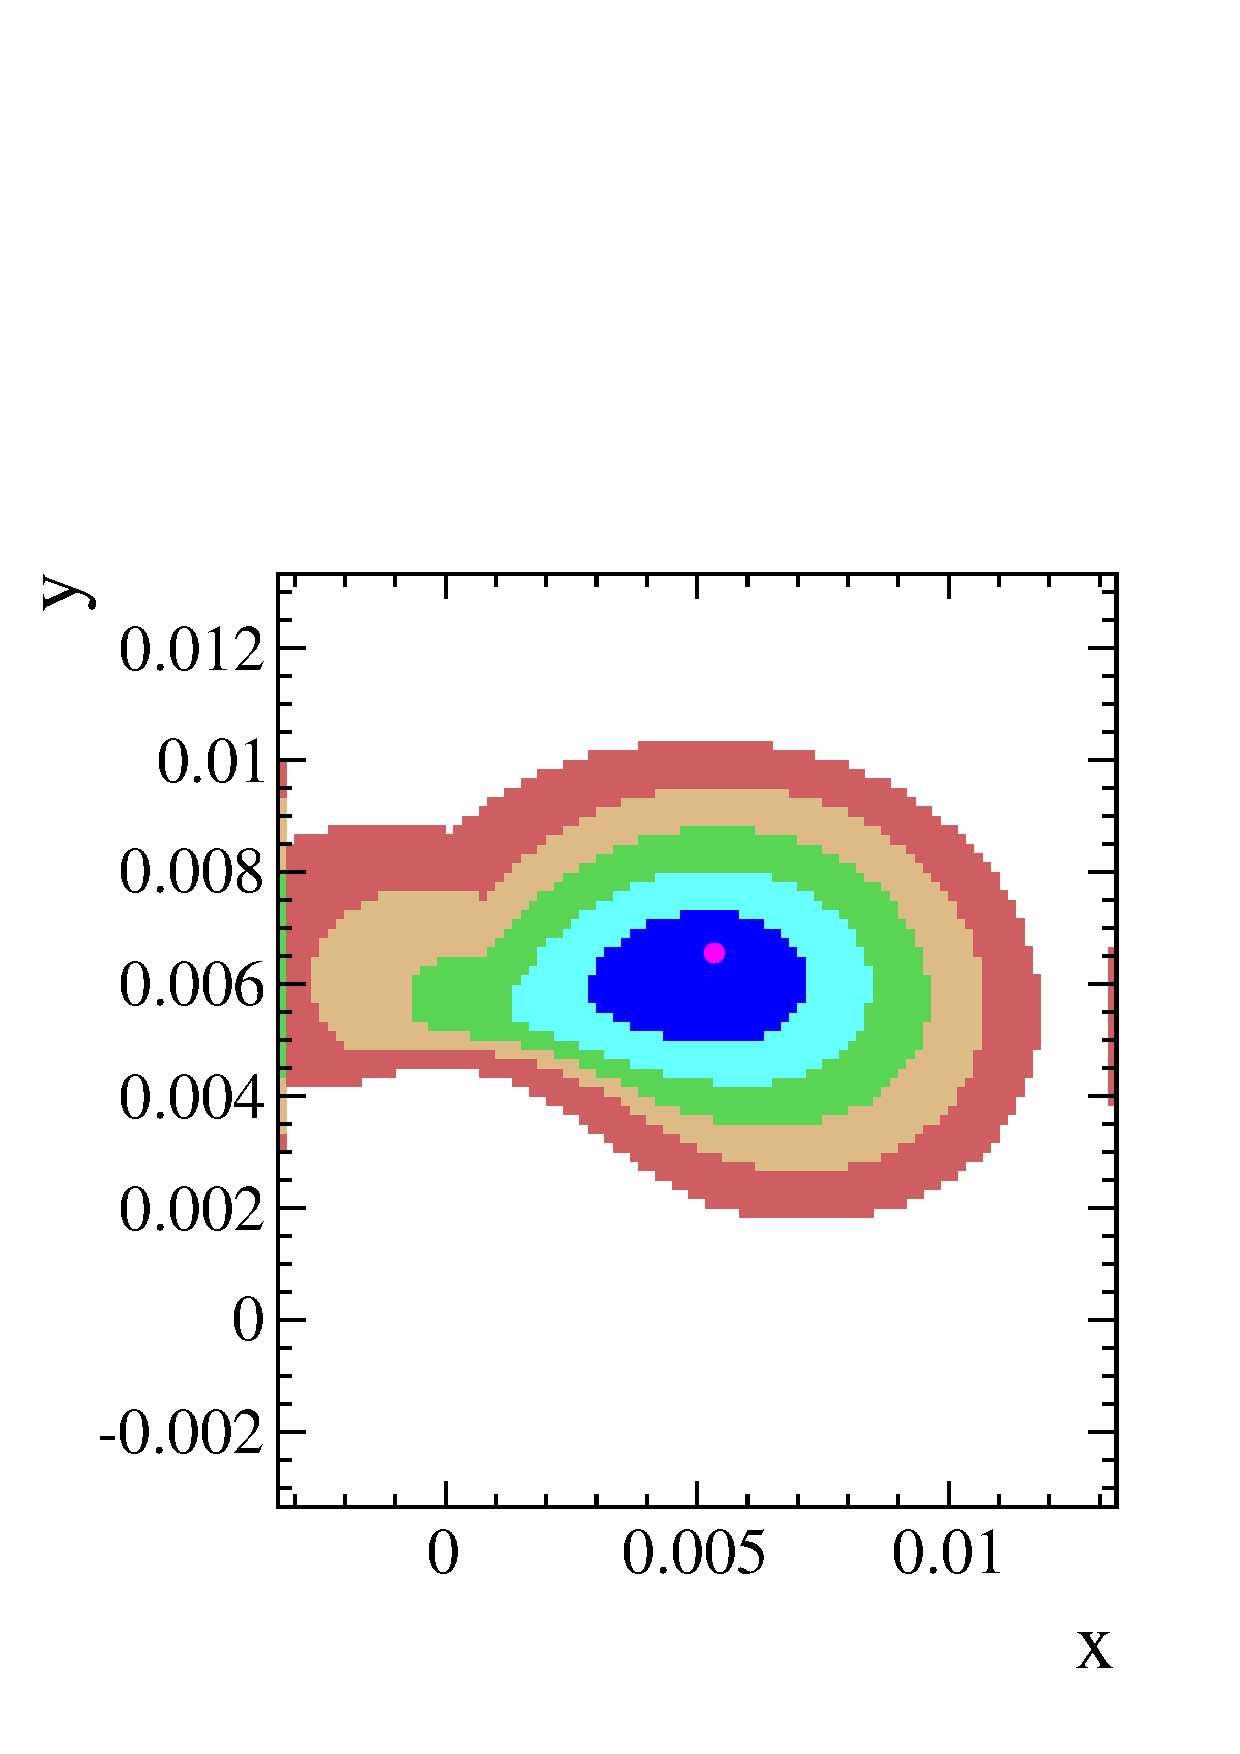
\includegraphics[width=\textwidth]{finalplot_nodcpv___hfag_agamma.pdf}
      \caption{Two dimensional error ellipses for x and y from fit to all data except LHCb $A_\Gamma$.}
      \label{fig:all_nodcpv_no_lhcb_agamma}
    \end{subfigure}%
    \\
%%%%%%%%%
    %\hspace{2mm}
    \begin{subfigure}[b]{0.4\textwidth}
      \centering
      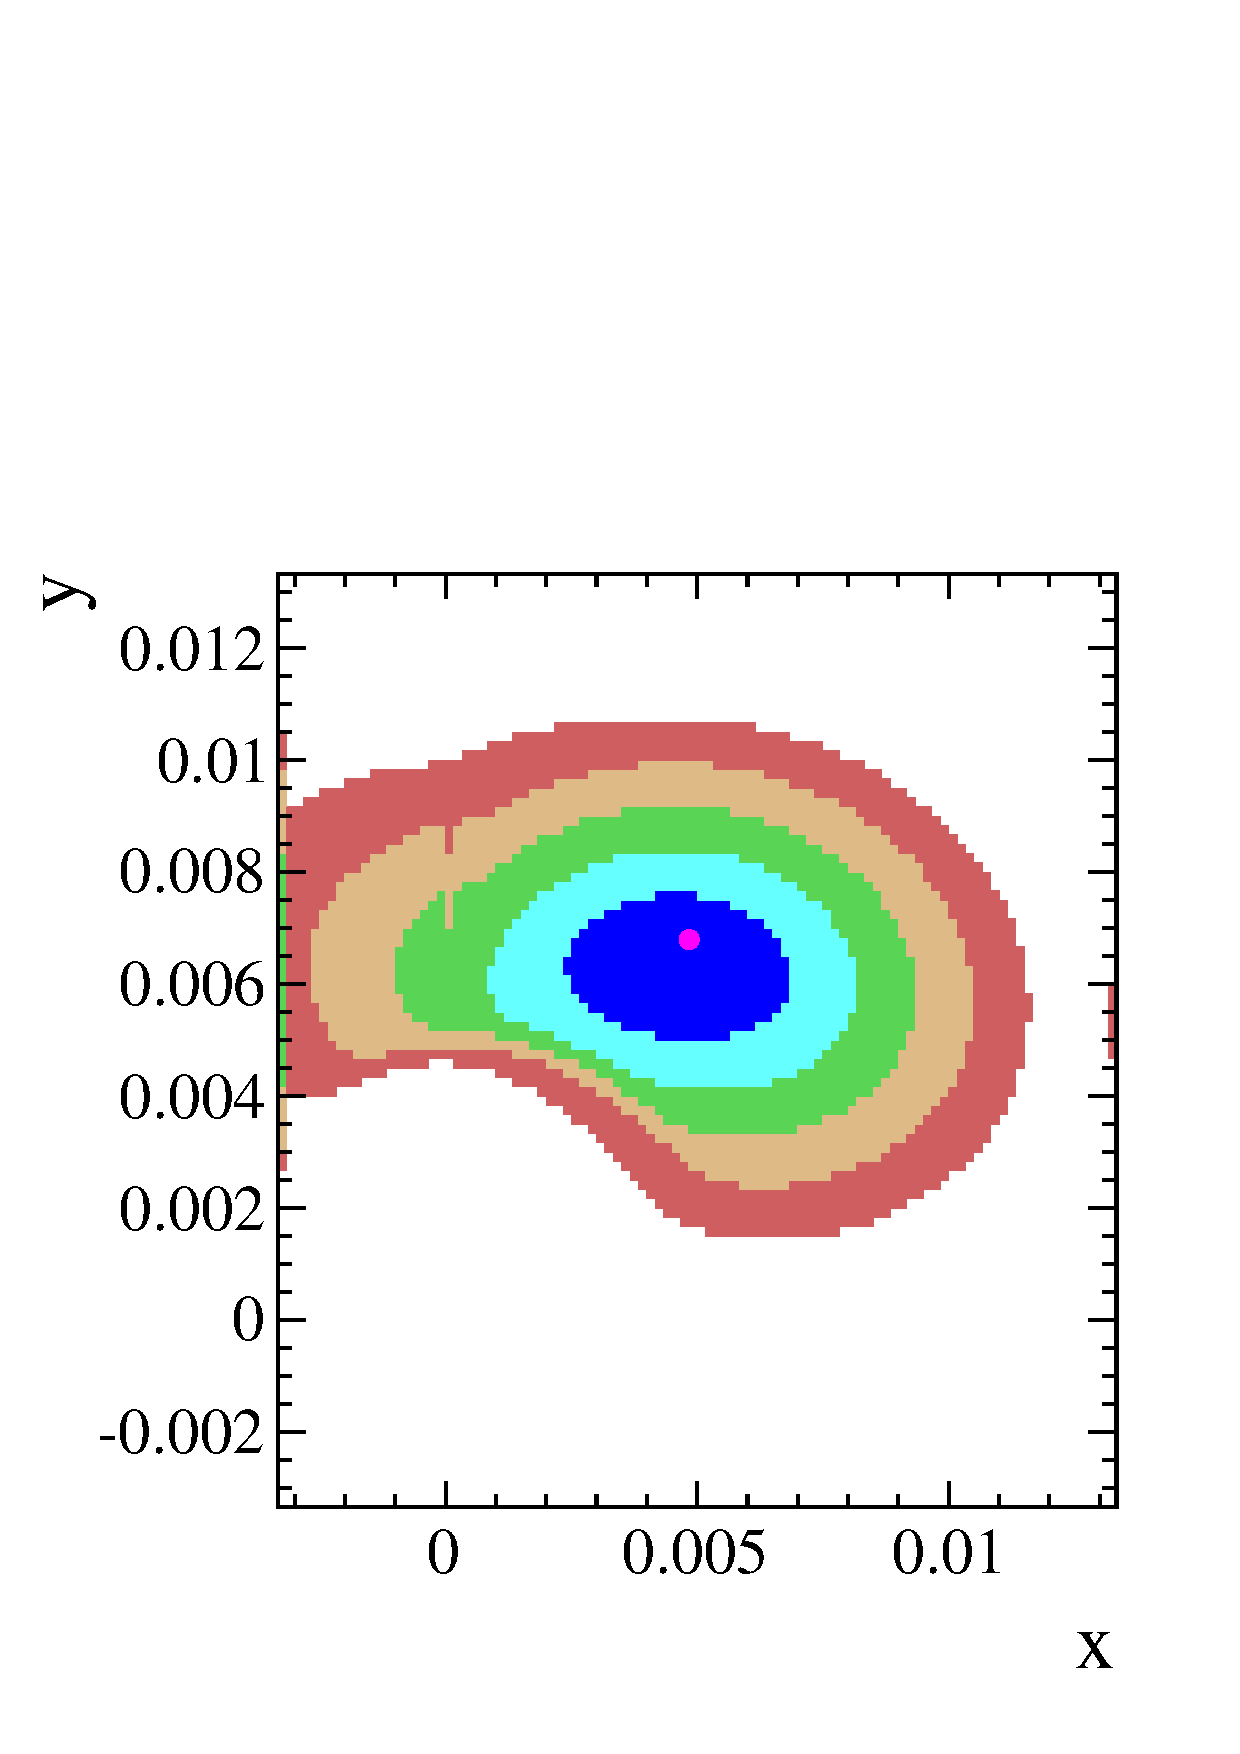
\includegraphics[width=\textwidth]{finalplot_nodcpv__nobelle_babar_.pdf}
      \caption{x vs y for Data excluding Belle and Babar $K \pi$ results.}
      \label{fig:nodcpv_no_belle_babar}
    \end{subfigure}%
    \hspace{2mm}
    \begin{subfigure}[b]{0.4\textwidth}
      \centering
      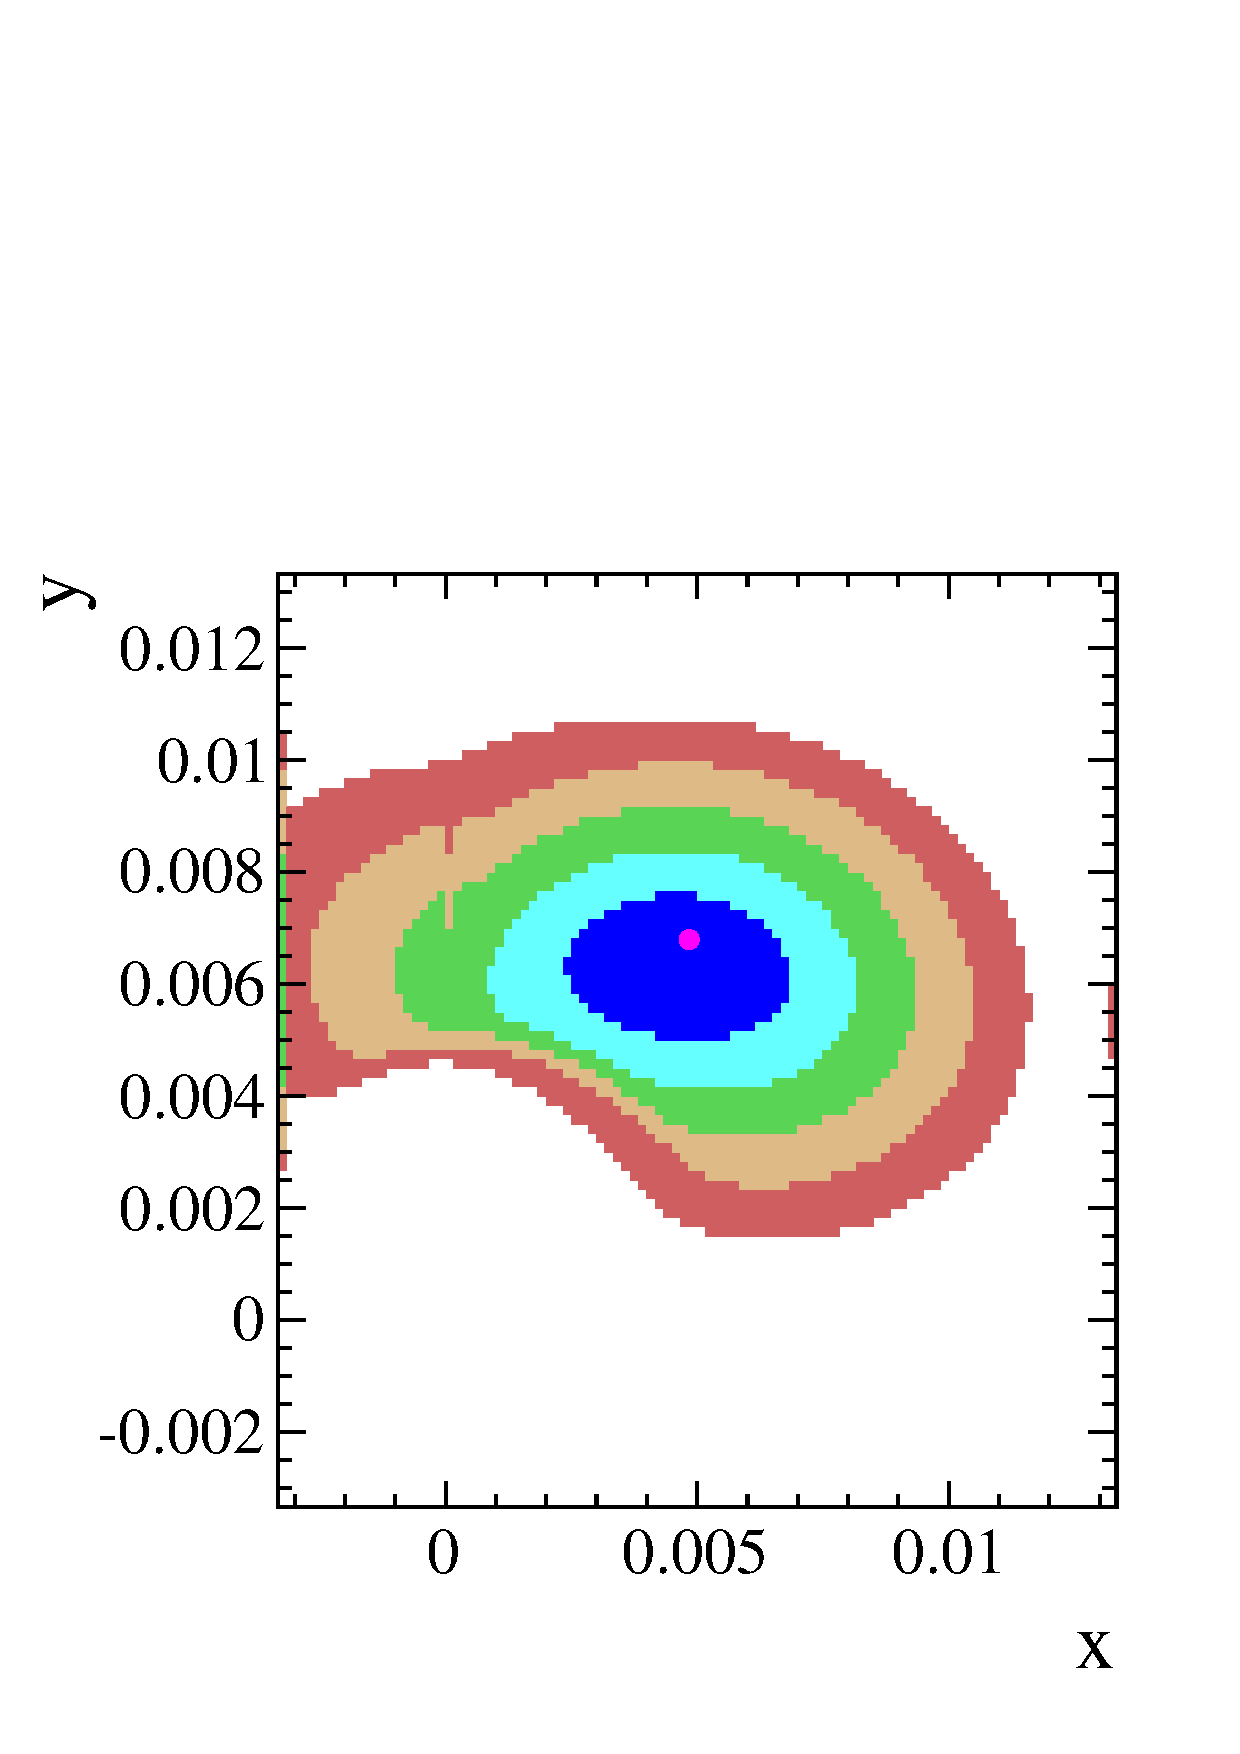
\includegraphics[width=\textwidth]{finalplot_nodcpv__nobelle_babar__hfag_agamma.pdf}
      \caption{Two dimensional error ellipses for x and y for No Direct CPV, excluding Belle and BaBar $K\pi$ results, and excluding LHCb $A_\Gamma$.}
      \label{fig:nodcpv_no_belle_babar_no_lhcb_agamma}
    \end{subfigure}%
    %\vspace*{-1.0cm}
  \end{center}
  \caption{Two dimensional error ellipses of fit for All CPV including differing sets of data for $x$ vs $y$. The biggest differences come from including the CDF result, which elongates the error ellipses. The differing colors represent the 1-5$\sigma$ contours.}
  \label{fig:xy_nodcpv_variations}
\end{figure}


%%%%%%%%%%%%%%%%%%%%%%%%%%%%%%%%%%%%%%%%%%%%
\subsection{All CP Violation Allowed}
Table~\ref{table:allcpv_output_table} lists the results of the global All CP Violation
allowed fit. Again, the latter columns list the differing subsets of the data to explore
the variation in global $\chi^2/$ndf. The most noticable difference between all fits
is the evaluation of $x$, which varies quite a bit with the inclusion of differing datasets.


%%%%%%%%%%%%%%% XY %%%%%%%%%%%%%%%%%%%%%%%%%
%\begin{table}[htdp]
%\begin{tiny}

\begin{center}
\resizebox{16cm}{!} {
\begin{tabular}{|c||c||c||c||c|}
\hline
& All Measurements & No Belle, BaBar& No Belle, BaBar, $A_{\Gamma\text{ LHCb}}$ & No Belle, BaBar, CDF,$A_{\Gamma\text{ LHCb}}$ \\ \hline

$x(\times10^{-3})$& $3.737\pm 1.630$ &$4.817\pm1.688$ &$4.772\pm1.685$ &$4.601\pm1.664$ \\ \hline

$y(\times10^{-3})$& $6.128 \pm 0.743$ & $6.868\pm 0.984$&$6.908\pm0.963$ & $6.956\pm0.867$\\ \hline

$\delta_{K\pi}(\times10^{-1})[\text{rad}]$& $ 1.146\pm 2.127$ & $3.246\pm1.935$& $3.329\pm1.891$& $3.250\pm1.756$\\ \hline

$\phi(\times10^{-1})[\text{rad}]$& $-0.642\pm1.255 $ &$-0.623\pm 1.055$&$-0.651\pm1.046$ & $-1.534\pm1.712$\\ \hline

$R_D^-(\times10^{-3})$& $3.501 \pm 0.040$&$3.568\pm 0.049$& $3.567\pm0.049$&$3.582\pm0.055$ \\ \hline

$R_D^+(\times10^{-3})$& $3.496\pm 0.036$ & $3.547\pm 0.044$ & $3.548\pm 0.043$&$3.533\pm0.046$ \\ \hline

$|q/p|(\times10^{-1})$& $9.631\pm 0.693$& $9.513\pm0.823$&$9.474\pm0.800$ & $8.880\pm1.082$\\ \hline

$\chi^2/ndf$& 59.9402/29 &18.8317/11 & 19.1817/14 & 7.72181/9\\ \hline

\end{tabular}
}
\end{center}
\caption{Output of the All CP Violation allowed global fit. Different Columns list 
differing subsets of data included in the fit.}
\label{table:allcpv_output_table}
%\end{tiny}
\end{table}%

%\begin{figure}[htb]
%  \begin{center}
%    \begin{subfigure}[b]{0.4\textwidth}
%      \centering
%      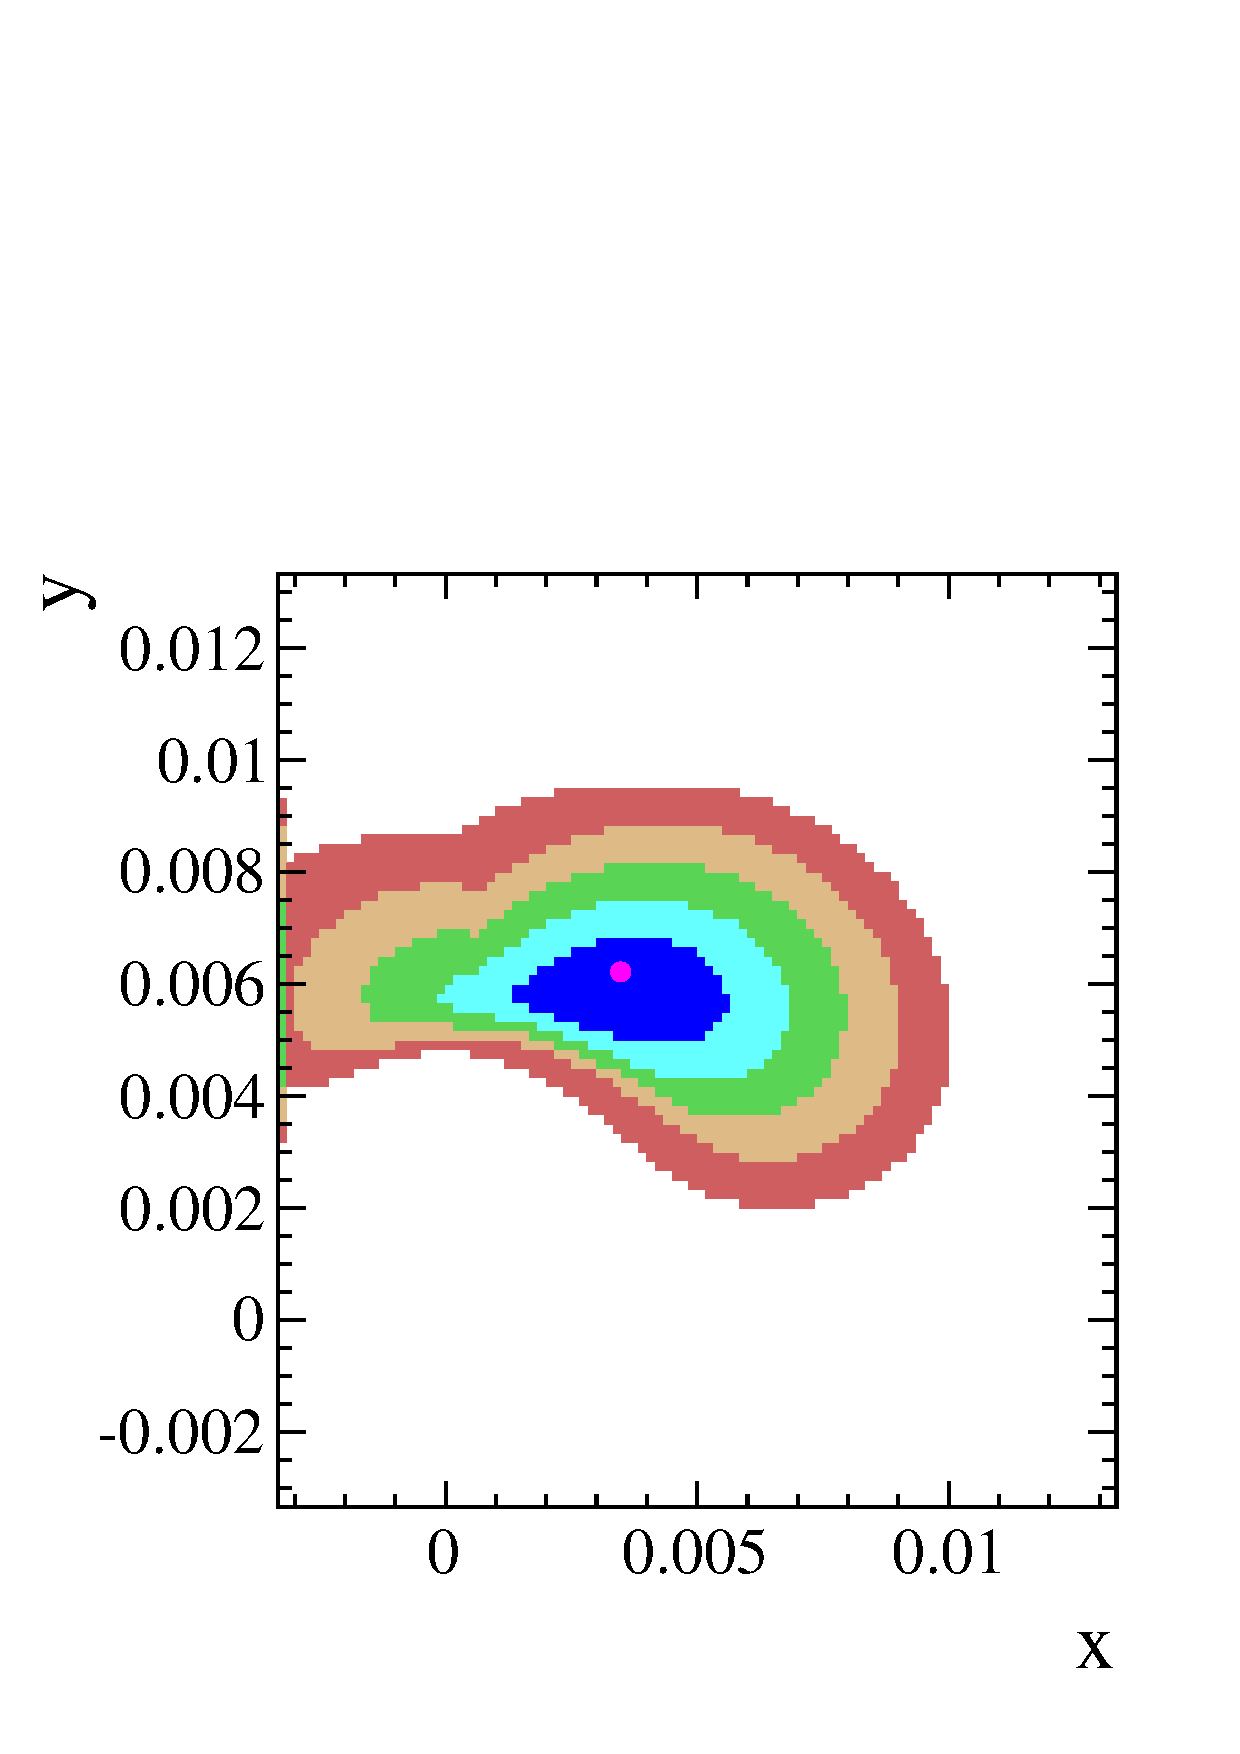
\includegraphics[width=\textwidth]{finalplot_allcpv_no_belle_babar_graph_hfag_agamma.pdf}
%      \caption{Two dimensional error ellipses for x and y from fit excluding Belle and BaBar $K\pi$ results. Does not include latest $A_\Gamma$ result of LHCb.}
%      \label{fig:xy_all_cpv_no_agamma}
%    \end{subfigure}%
%    \hspace{2mm}
%    \begin{subfigure}[b]{0.4\textwidth}
%      \centering
%      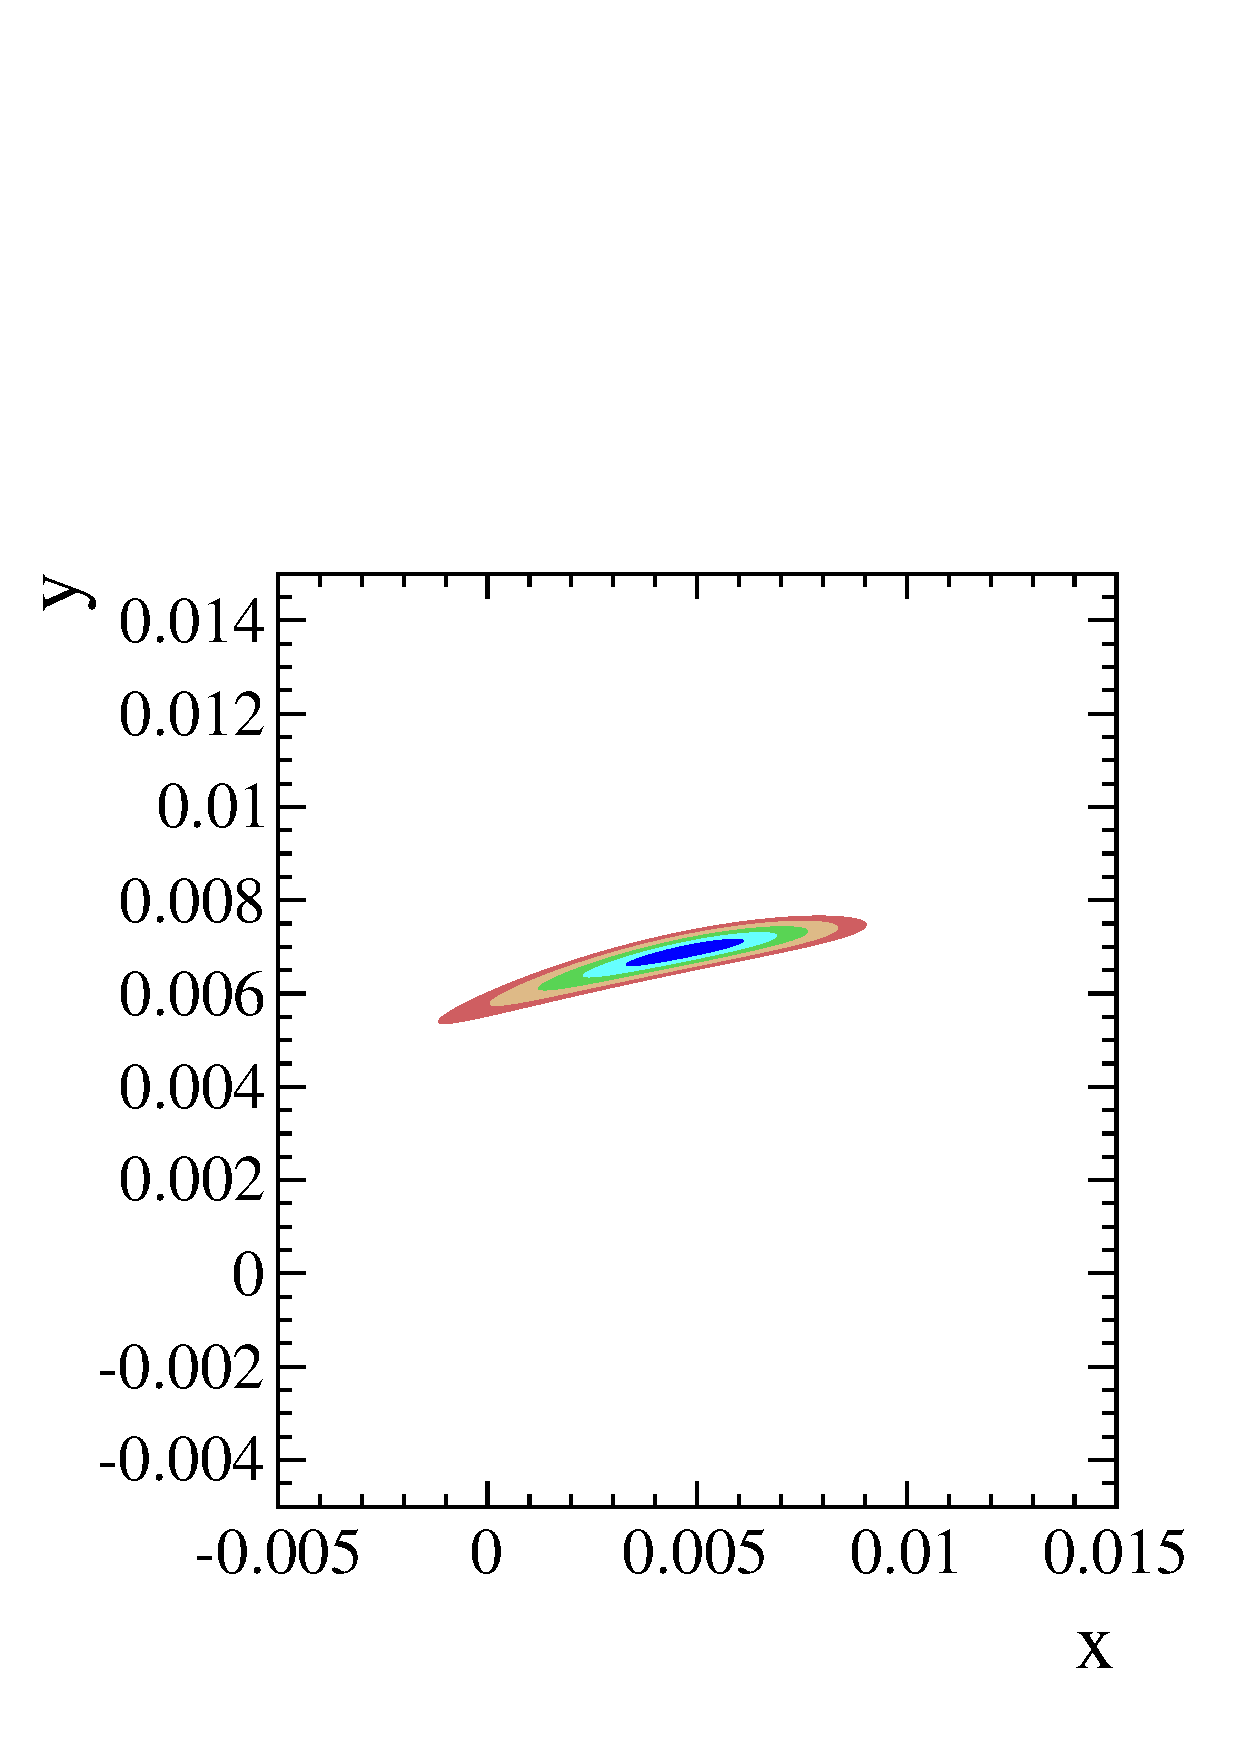
\includegraphics[width=\textwidth]{finalplot_allcpv_no_belle_babar_graph_lhcb_agamma.pdf}
%      \caption{Two dimensional error ellipses for x and y from fit excluding Belle and BaBar $K\pi$ results. Include latest $A_\Gamma$ result of LHCb.}
%      \label{fig:xy_all_cpv_with_agamma}
%    \end{subfigure}%
%    \\
%%%%%%%%%%
%    %\hspace{2mm}
%    \begin{subfigure}[b]{0.4\textwidth}
%      \centering
%      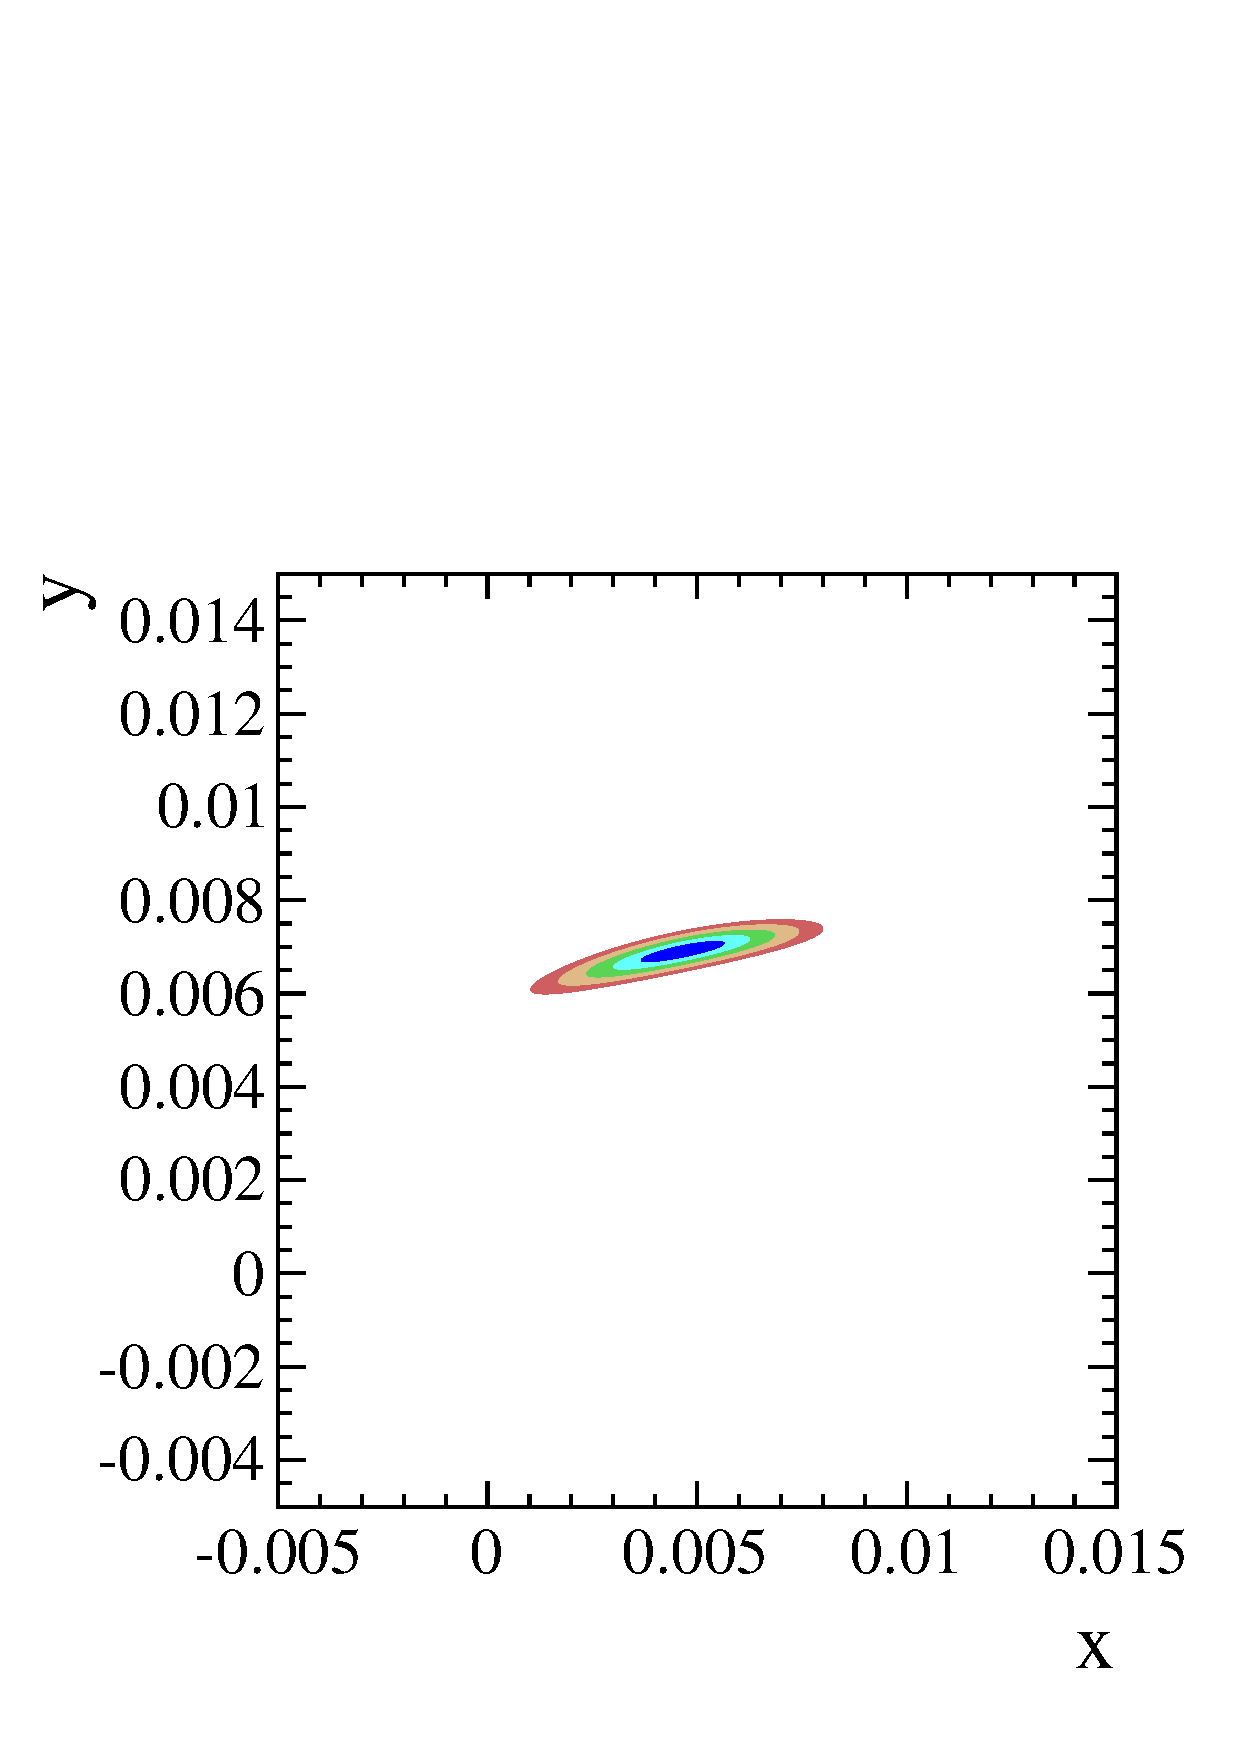
\includegraphics[width=\textwidth]{finalplot_allcpv_no_belle_babar_cdf_graph_hfag_agamma.pdf}
%      \caption{Two dimensional error ellipses for x and y from fit excluding Belle, BaBar and CDF $K\pi$ results. Does not include latest $A_\Gamma$ result of LHCb.}
%      \label{fig:xy_all_cpv_no_agamma}
%    \end{subfigure}%
%    \hspace{2mm}
%    \begin{subfigure}[b]{0.4\textwidth}
%      \centering
%      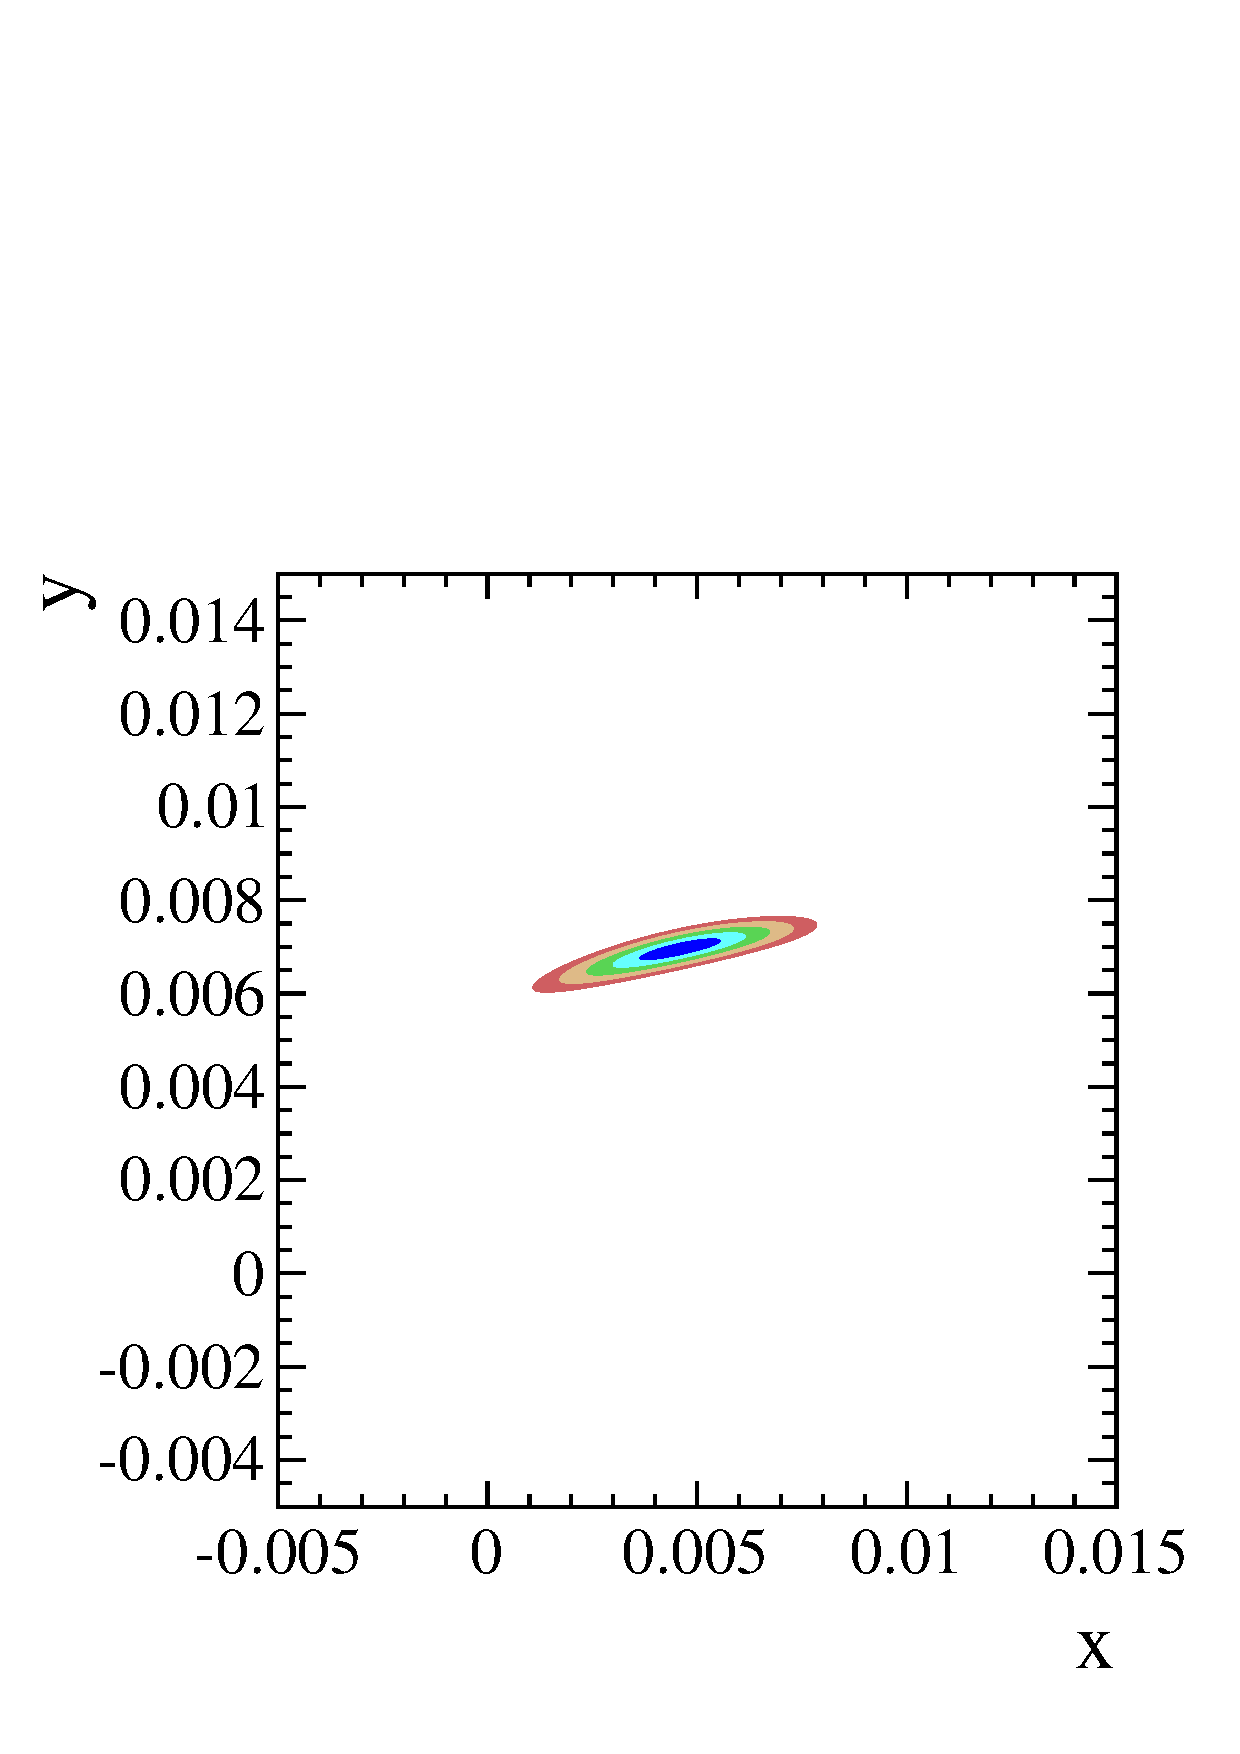
\includegraphics[width=\textwidth]{finalplot_allcpv_no_belle_babar_cdf_graph_lhcb_agamma.pdf}
%      \caption{Two dimensional error ellipses for x and y from fit excluding Belle, BaBar and CDF $K\pi$ results. Include latest $A_\Gamma$ result of LHCb.}
%      \label{fig:xy_all_cpv_with_agamma}
%    \end{subfigure}%
%    %\vspace*{-1.0cm}
%  \end{center}
%  \caption{Two dimensional error ellipses of fit for All CPV including differing sets of data for $x$ vs $y$. The biggest differences come from including the CDF result, which elongates the error ellipses. The differing colors represent the 1-5$\sigma$ contours.}
%  \label{fig:xy_all_variations}
%\end{figure}

%%%%%%%%%%%%%%%% Q/P %%%%%%%%%%%%%%%%%%%%%%%%%%%%%%%%%%%%
\begin{figure}[tb]
  \begin{center}
    \begin{subfigure}[b]{0.4\textwidth}
      \centering
      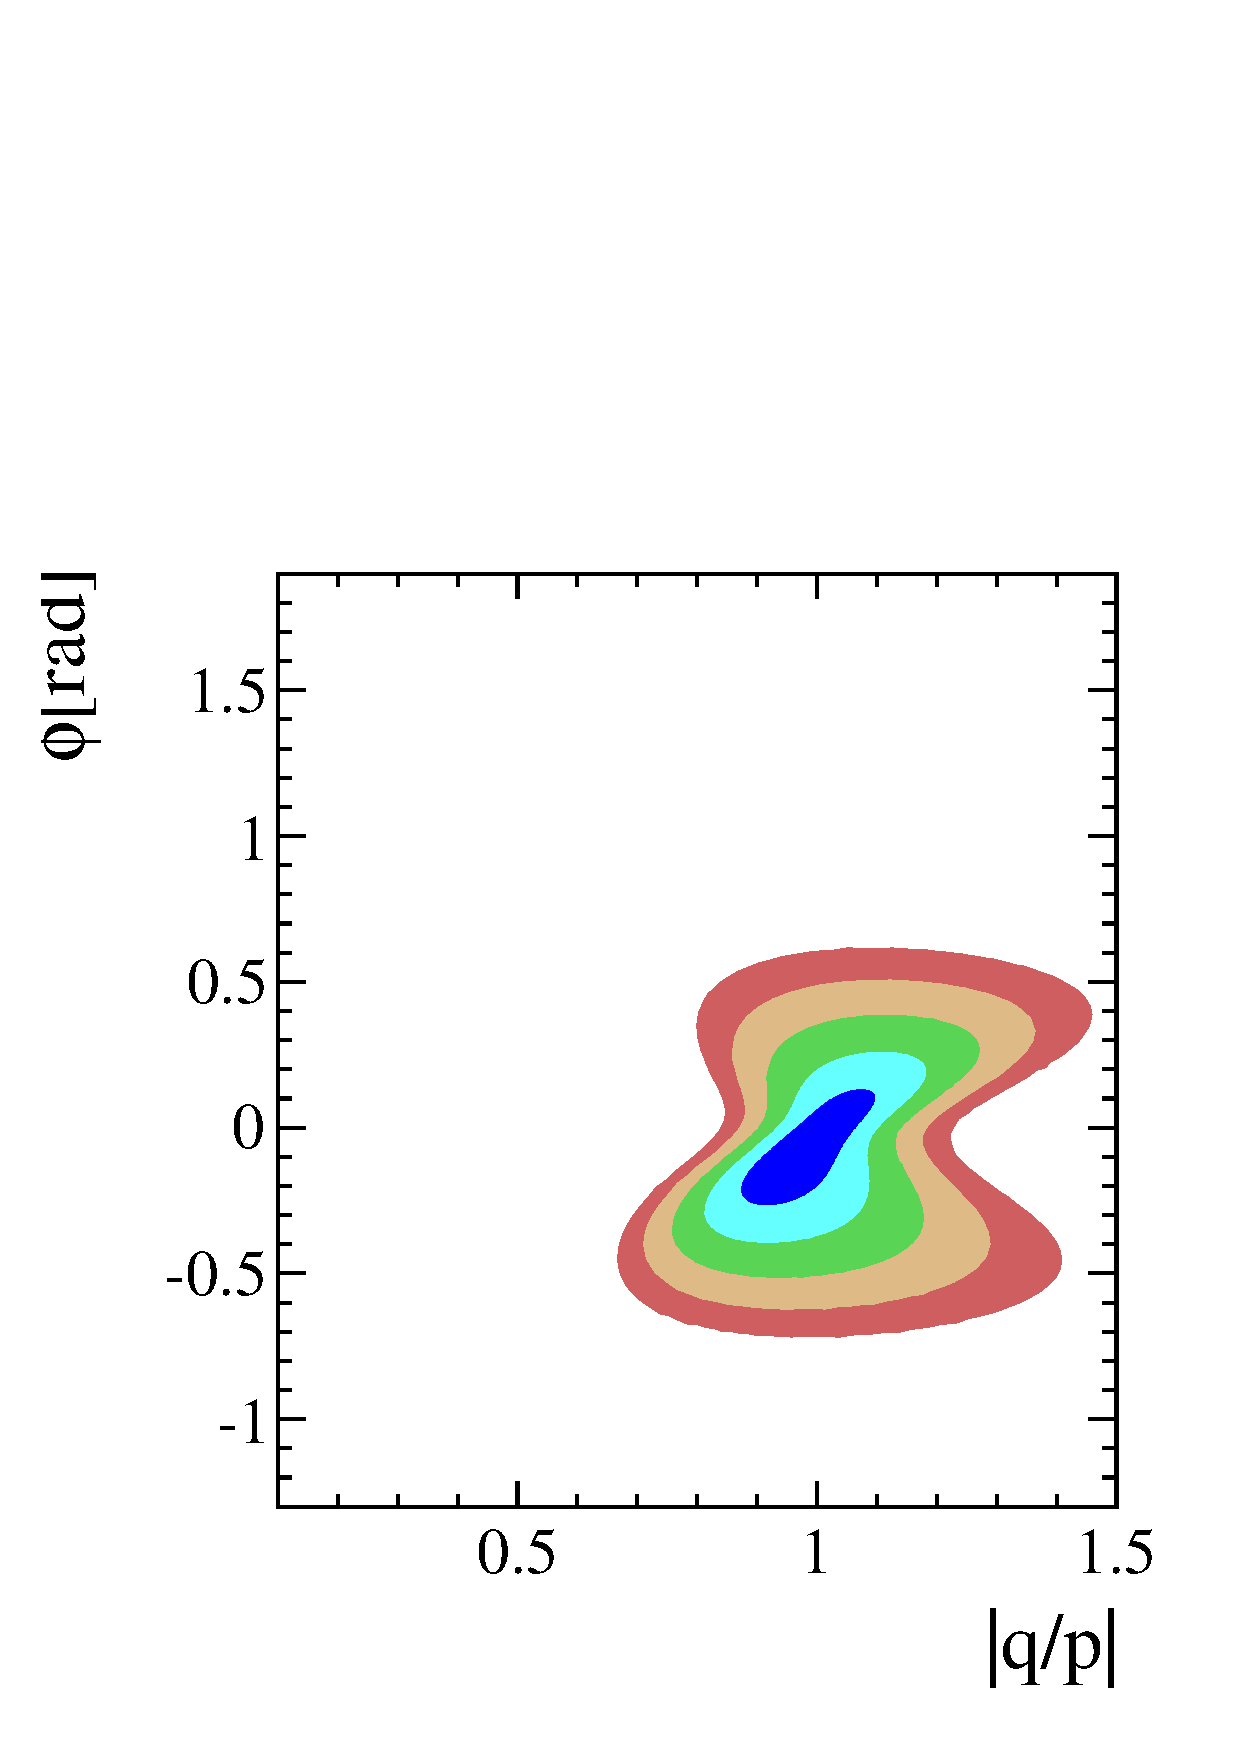
\includegraphics[width=\textwidth]{finalplot_allcpv_no_belle_babar_graph_qop_phi_hfag_agamma.pdf}
      \caption{Two dimensional error ellipses for x and y from fit excluding Belle and BaBar $K\pi$ results. Does not include latest $A_\Gamma$ result of LHCb.}
      \label{fig:xy_all_cpv_no_agamma}
    \end{subfigure}% 
    \hspace{2mm}
    \begin{subfigure}[b]{0.4\textwidth}
      \centering
      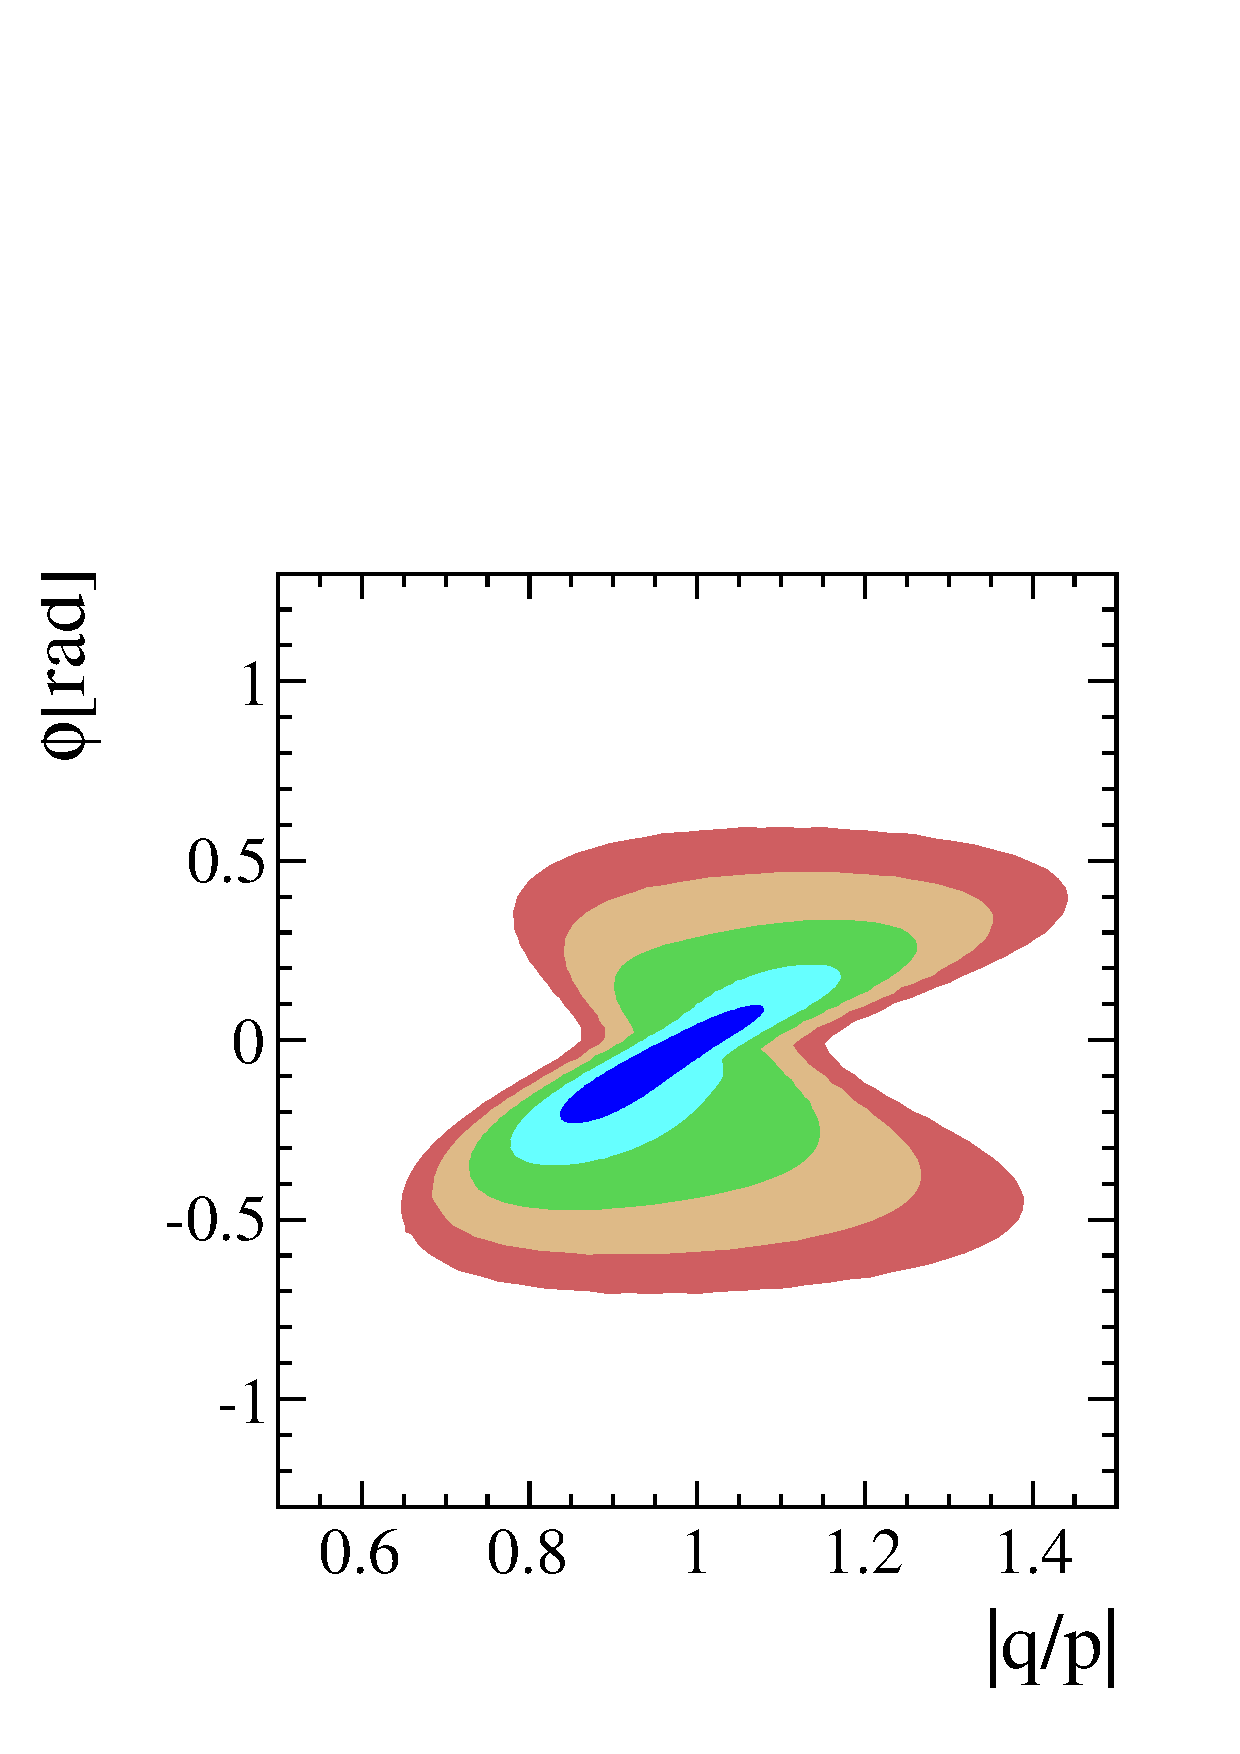
\includegraphics[width=\textwidth]{finalplot_allcpv_no_belle_babar_graph_qop_phi_lhcb_agamma.pdf}
      \caption{Two dimensional error ellipses for x and y from fit excluding Belle and BaBar $K\pi$ results. Include latest $A_\Gamma$ result of LHCb.}
      \label{fig:xy_all_cpv_with_agamma}
    \end{subfigure}%
%%%%%%%%%
        \\
    \begin{subfigure}[b]{0.4\textwidth}
      \centering
      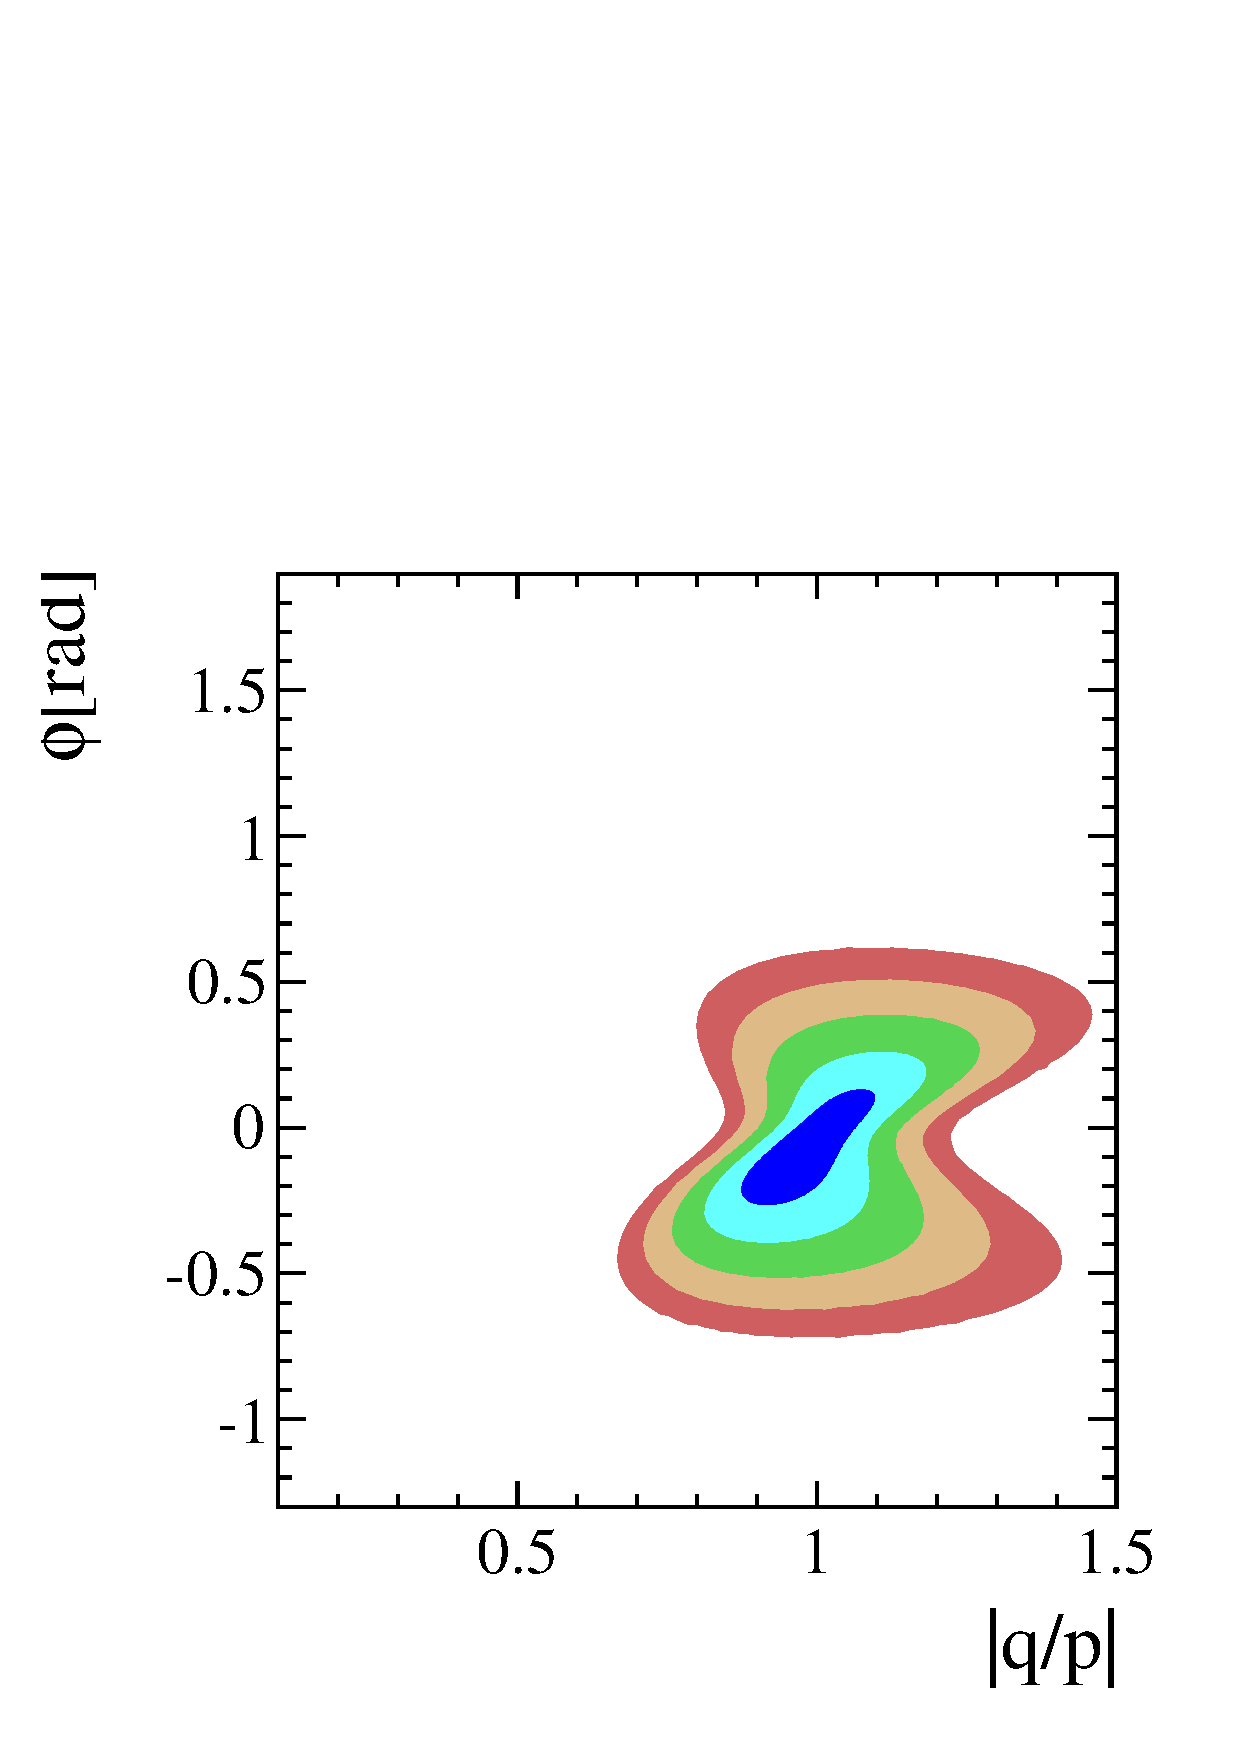
\includegraphics[width=\textwidth]{finalplot_allcpv_no_belle_babar_cdf_graph_qop_phi_hfag_agamma.pdf}
      \caption{Two dimensional error ellipses for x and y from fit excluding Belle, BaBar and CDF $K\pi$ results. Does not include latest $A_\Gamma$ result of LHCb.}
      \label{fig:xy_all_cpv_no_agamma}
    \end{subfigure}%
    \hspace{2mm}
    \begin{subfigure}[b]{0.4\textwidth}
      \centering
      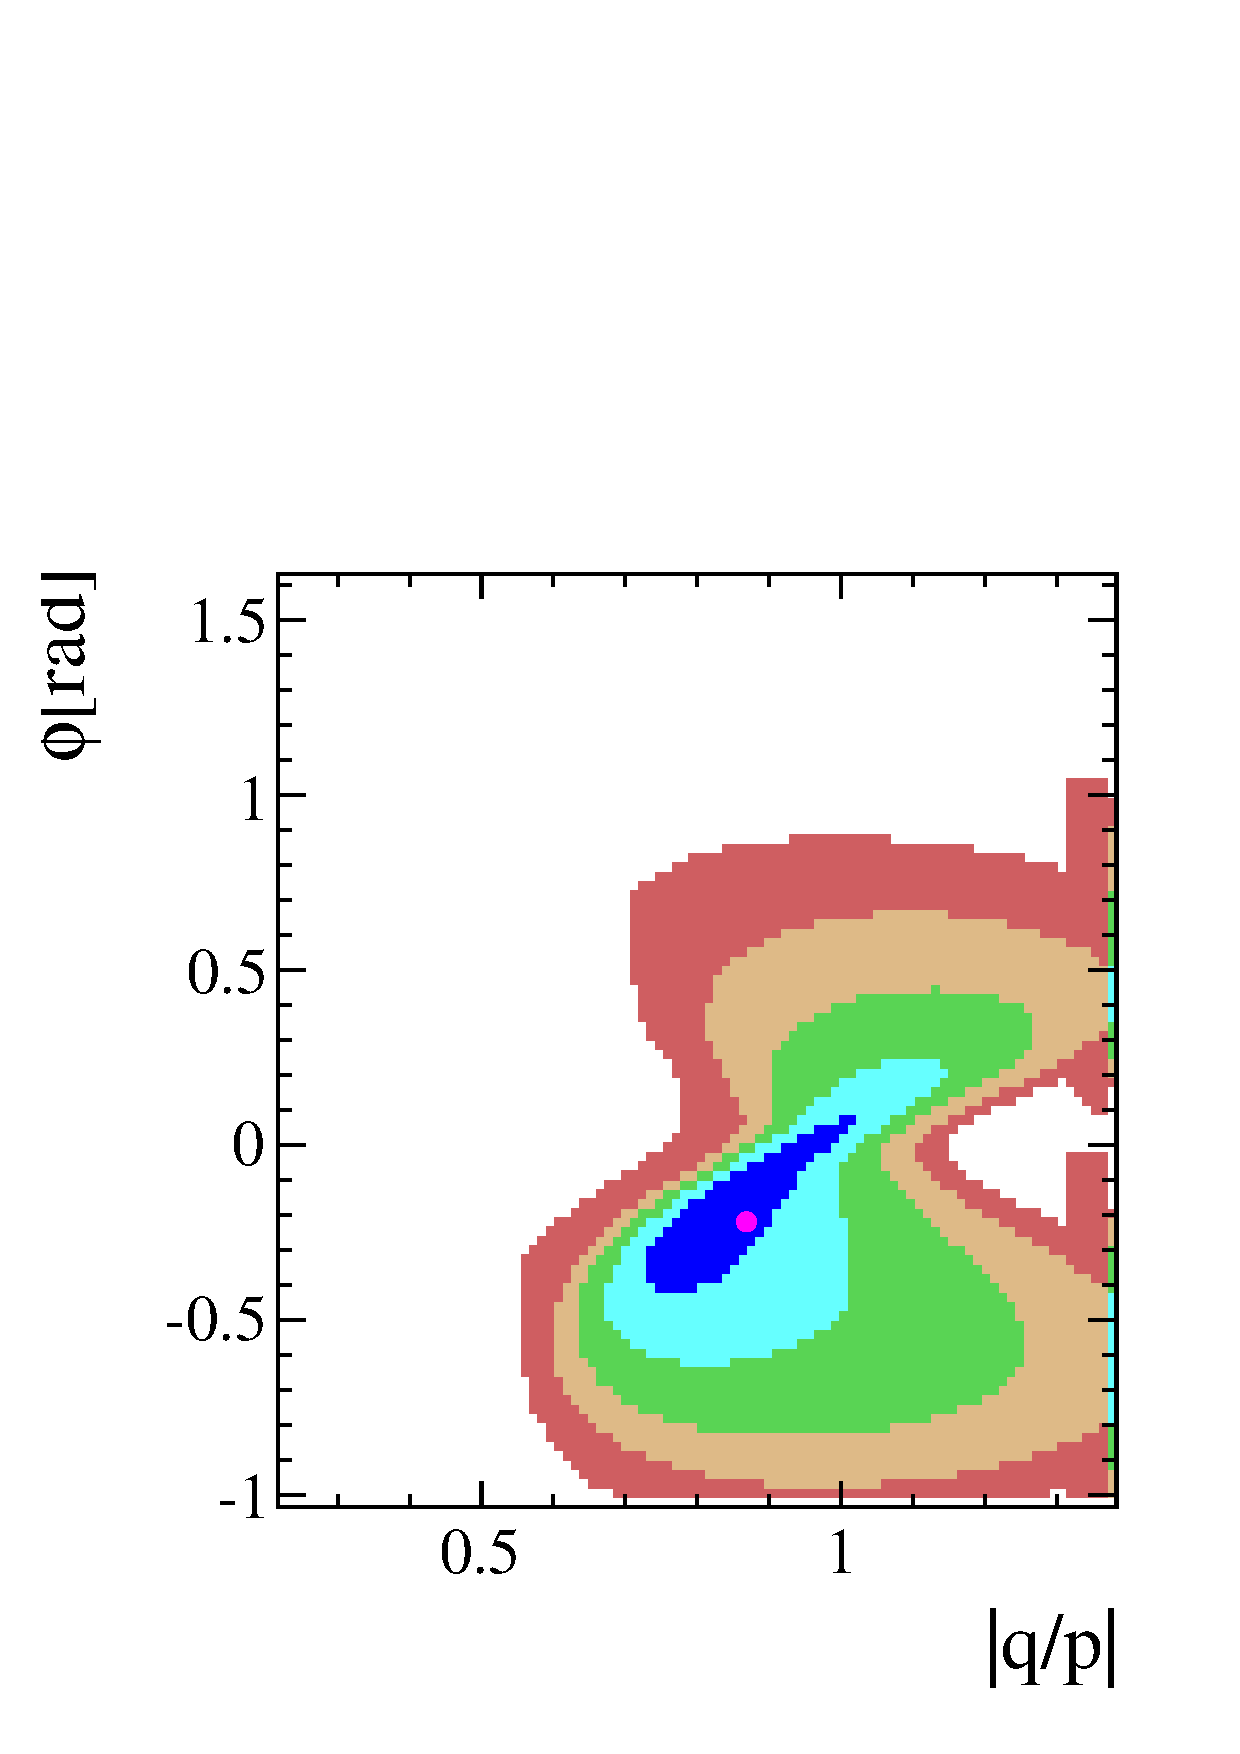
\includegraphics[width=\textwidth]{finalplot_allcpv_no_belle_babar_cdf_graph_qop_phi_lhcb_agamma.pdf}
      \caption{Two dimensional error ellipses for x and y from fit excluding Belle, BaBar and CDF $K\pi$ results. Include latest $A_\Gamma$ result of LHCb.}
      \label{fig:xy_all_cpv_with_agamma}
    \end{subfigure}%
    %\vspace*{-1.0cm}
  \end{center}
  \caption{Two dimensional error ellipses of fit for All CPV including differing sets of data for $\phi$ vs $q/p$. The biggest differences come from including the CDF result, which elongates the error ellipses. The differing colors represent the 1-5$\sigma$ contours.}
  \label{fig:xy_all_variations}
\end{figure}

\subsection{All CP Violation Allowed, Fit for $x_{12},y_{12},\phi_{12}$}
Table~\ref{table:allcpv_output_table_alex} lists the results for the All CPV allowed fit with the substitution of $x$ and $y$ for the underying parameters $x_{12},y_{12}$ and $\phi_{12}$. 
\begin{table}[htdp]
%\begin{tiny}

\begin{center}
\resizebox{16cm}{!} {
\begin{tabular}{|c||c||c||c||c|}
\hline
& All Measurements & No Belle, BaBar& No Belle, BaBar, $A_{\Gamma\text{ LHCb}}$ & No Belle, BaBar, CDF,$A_{\Gamma\text{ LHCb}}$ \\ \hline

$x_{12}(\times10^{-3})$&$ 3.789\pm1.627$  & $4.842\pm1.693$&$4.842\pm1.693$ & $4.853\pm1.694$\\ \hline

$y_{12}(\times10^{-3})$&$ 6.365\pm 0.953$  &$6.851\pm0.099$ & $6.851\pm 0.994$&$6.863\pm0.994$ \\ \hline

$\delta_{K\pi}(\times10^{-1})[\text{rad}]$&$1.855\pm 2.523$ & $3.237\pm1.949$& $3.237\pm1.949$&$3.191\pm1.950$ \\ \hline

$\phi_{12}(\times10^{-2})[\text{rad}]$&$-0.304\pm4.277$ &$-0.210\pm3.416$ & $-0.210\pm3.416$&$-0.249\pm3.380$ \\\hline

$R_D^-(\times10^{-3})$&$3.501\pm0.038$ & $3.556\pm0.043$& $3.556\pm0.043$& $3.556\pm0.043$\\ \hline

$R_D^+(\times10^{-3})$& $3.505\pm0.038$& $3.558\pm0.043$& $3.558\pm0.043$& $3.558\pm0.043$\\ \hline

$\chi^2/ndf$& 50.73/27&  19.5825/15& 19.5825/15& 8.62343/12\\ \hline

\end{tabular}
}
\end{center}
\caption{Output of the All CP Violation allowed global fit when fitting for the 
underlying parameters $x_{12}$ and $y_{12}$. Different Columns list 
differing subsets of data included in the fit.}
\label{table:allcpv_output_table_alex}
%\end{tiny}
\end{table}%


\section{Conclusion}



\label{lastpage}
\end{document}
